\documentclass[10pt]{style/sigplanconf}
%\documentclass[10pt]{style/sigplanconf}

\input{tweaks.tex}

%%% AEC BADGE THINGY %%%
\usepackage[firstpage]{draftwatermark}
\SetWatermarkText{\hspace*{8in}\raisebox{4.4in}{
\includegraphics[scale=0.1]{aec/aec-badge.eps}}}
\SetWatermarkAngle{0}
%%%%%%%%%%%%%%%%%%%%%%%%

\begin{document}

\special{papersize=8.5in,11in}
\setlength{\pdfpageheight}{\paperheight}
\setlength{\pdfpagewidth}{\paperwidth}

% \toappear{}
\exclusivelicense
\conferenceinfo{OOPSLA~'15}{October 25-30 2015, Pittsburgh, PA, USA}
\copyrightyear{2015}
\copyrightdata{978-1-4503-3689-5/15/10}
\doi{2814270.2814271}

\titlebanner{DRAFT - Please do not distribute}
\preprintfooter{DRAFT - Please do not distribute}

\title{\Automating Ad hoc Data Representation Transformations}

\authorinfo{Vlad Ureche$^\dagger$
\and Aggelos Biboudis$^*$
\and Yannis Smaragdakis$^*$
\and Martin Odersky$^\dagger$} {
$^\dagger$École polytechnique fédérale de Lausanne, Switzerland: \texttt{\{first.last\}@epfl.ch}\qquad \\
$^*$University of Athens, Greece: \texttt{\{biboudis, smaragd\}@di.uoa.gr}
}

\maketitle

% Body of the paper

\begin{abstract}

Generics on the Java platform are compiled using the erasure transformation, which only supports by-reference values. This causes slowdowns when generics operate on primitive types, such as integers, as they have to be transformed into reference-based objects.

Project Valhalla is an effort to remedy this problem by specializing classes at load-time so they can efficiently handle primitive values. In its current early prototype\footnote{As of August 2015 \cite{valhalla-model2-announcement,valhalla-model2-implementation}.\vspace{-1em}}, the Valhalla compilation scheme limits the interaction between specialized and erased generics, thus preventing certain useful code patterns from being expressed.

Scala has been using compile-time specialization for 6 years and has three generics compilation schemes working side by side. In Scala, programmers are allowed to write code that freely exercises the interaction between the different compilation schemes, at the expense of introducing subtle performance issues. Similar performance issues can affect Valhalla-enabled bytecode, whether the code was written in Java or translated from other JVM languages.

In this context we explain how we help programmers avoid these performance regressions in the miniboxing transformation: (1) by issuing actionable performance advisories that steer programmers away from performance regressions and (2) by providing alternatives to the standard library constructs that use the miniboxing encoding, thus avoiding the conversion overhead.

\vspace{-0.5em}

\keywords{generics, specialization, miniboxing, backward compatibility, data representation, performance, Java, bytecode, JVM}

\vspace{-0.5em}

\end{abstract}

% \section*{Crash course to Vlad's \LaTeX tweaks}

\vlad{Feel free to make changes directly on the paper.} If you want to start a discussion, you can use |\yannis{text}| , |\aggelos{text}| or |\dima{text}|. The comment above was made using |\vlad{...}|. And you can change your color in the |tweaks.tex| file. Another two things:



\noindent Code: use |\begin{lstlisting-nobreak}|. Inside the code you can highlight using backquotes |`|:

\begin{lstlisting-nobreak}
  def `foo`: Int = `3`
\end{lstlisting-nobreak}

\noindent By the way, don't try to highlight starting from the first character, it looks ugly:

\begin{lstlisting-nobreak}
  `def foo`: Int = `3`
\end{lstlisting-nobreak}

\noindent Verbatim: use straight bars, like \verb=|=, e.g: \verb=|verbatim text|=.

My own comment, which does not reflect the views of my employer: The Springer template sucks compared to |sigplan.cls|!
\section{Introduction}
\label{sec:intro}

Generics on the Java platform are compiled using the erasure transformation \cite{java-erasure}, which allows them to be fully backward compatible with pre-generics bytecode. Unfortunately, this also means that they only handle by-reference values (objects) and not primitive types. Thus, primitive values such as bytes and integers have to be converted to heap objects each time they interact with generics. This conversion, known as boxing, compromises the execution performance and increases the heap footprint, forcing Java to lag behind lower-level languages such as C or C++.

The performance drawbacks of erasure are currently being addressed in Project Valhalla\footnote{The Valhalla Project is still in its infancy, but early prototypes are openly available and the hard goals have been clearly defined in \cite{goetz-specialization, rose-value-classes-tearing, rose-value-classes-vm}.}, an important undertaking led by the Java platform architects and aimed at providing unboxed generics for Java and other JVM languages. The updated bytecode format in Project Valhalla will include the necessary type information to allow load-time class specialization, effectively creating different versions of classes that directly support primitive types. This load-time transformation approach is also employed by the .NET framework \cite{dot-net-generics,dot-net-generics-form} in order to implement generics.

Unlike .NET generics, which are always specialized, the current design of Project Valhalla, as of August 2015, makes it an explicit goal to have specialization as an opt-in transformation. This will allow the ecosystem to evolve smoothly from erased to specialized generics, allowing both erased and specialized classes to work side by side. However, in the current early prototype, there are still some restrictions: (1) erased code cannot handle specialized instances in a generic manner and, (2) abstracting over specialized classes using wildcard types \cite{valhalla-model2-announcement,valhalla-model2-implementation} pays the cost of boxing primitive types. This is shown in the following example:

\begin{lstlisting-nobreak}
// The Box class is specialized by virtue of its type
// parameter T being annotated with the "any" prefix:
public class Box<`any` T> {
  ...
  T getValue() { ... }
}

// The getBoxValue method is compiled with erasure
// since U is not marked with the "any" prefix:
static <U> U getBoxValue(Box<U> box) {
  return box.getValue();
}

// (1) erased code cannot handle specialized class
//        instances (the code will not compile):
getBoxValue(`new Box<int>(5)`);

// (2) abstracting over a specialized class leads to
//        boxing the value (any acts as a wildcard type):
Box<any> box = `new Box<int>(5)`;
System.out.println(`box.getValue()`); // boxes the value
\end{lstlisting-nobreak}

These two code patterns could easily be rewritten to make the code compile and to avoid the overhead of boxing. For the first pattern, adding the |any| prefix to the type parameter |U| of method |getBoxValue| would make it specialized as well, allowing it to handle the incoming argument. In the second pattern, the wildcard, which is equivalent to extending |Box<?>| to value types, could be replaced by the exact type, |Box<int>|, eliminating the overhead of boxing. Yet, in the general case, not all code can be changed at will, due to interactions, backward compatibility or because it resides in external libraries. Thus, a better solution would be to have erased and specialized generics interoperate, ideally without the overhead.

The Scala programming language, which also compiles to JVM bytecode, has had compile-time specialization for 6 years \cite{iuli-thesis, specialization-iuli} and currently has three mechanisms for compiling generics: erasure, specialization and a new arrival, miniboxing \cite{miniboxing}. In Scala, all three generics compilation schemes can be freely mixed:

\begin{lstlisting-nobreak}
// The Mbox class is miniboxed by virtue of the type
// parameter annotation (but could be specialized
// as well, using @specialized):
class Mbox[`@miniboxed` T](value: T) {
  def getValue(): T = ...
}

// The getMboxValue method is erased:
def getMboxValue[U](mbox: Mbox[U]): U = mbox.getValue()

// (1) erased code can handle specialized instances:
getMboxValue(`new Mbox[Int](5)`)
// (2) programmers can abstract over specializations:
val mbox: Mbox[_] = `new Mbox[Int](5)`
println(`mbox.getValue()`)
\end{lstlisting-nobreak}

Despite the uniform behavior, Scala does pay a hefty price for being able to freely mix code using the three generics compilation schemes: calls between different compilation schemes require boxing primitive values. The reason is that only boxed primitive values are understood by all three transformations. Furthermore, as we will see later on, instantiating a miniboxed (or specialized) class from erased code leads to the erased version being instantiated instead of its miniboxed (or specialized) equivalent, in turn leading to unexpected performance regressions.

In this paper, we show how we completely eliminate the unexpected slowdowns in the miniboxing transformation and, as a side effect, allow programmers to easily and robustly use miniboxing to speed up their programs. The underlying property we are after is that, inside hot loops and performance-sensitive parts of the program, all generic code uses the same compilation scheme, in this case, miniboxing. This way, primitive types are always passed using the same data representation, whether that's the miniboxed encoding (for miniboxing) or the unboxed representation (for specialization).

We show two approaches for harmonizing the compilation scheme across performance-sensitive code:

\textbf{Issuing actionable performance advisories} when compilation schemes do not match, allowing the programmer to harmonize them. For example, when a generic method takes a miniboxed class as a parameter and tries to call methods on it, we automatically generate performance advisories:

\begin{lstlisting-nobreak-nolang}
scala> def getMboxValue[U](mbox: Mbox[U]): U =
     |      mbox.getValue()
<console>:9: warning: The following code could benefit from miniboxing if the type parameter U of method getMboxValue would be marked as "@miniboxed U":
         mbox.getValue()
               ^
\end{lstlisting-nobreak-nolang}

Another problem that occurs frequently concerns library evolution: as a new compilation scheme arrives, it is best if all libraries start using it as soon as possible. However, backward compatibility prohibits changing the compilation scheme for the standard library, as it would break old bytecode. In Scala, we had this problem because many of the core language constructs, such as functions and tuples use specialization instead of miniboxing. Similarly, Java has as many as 20 manual specializations for the arity 1 lambda, such as |IntConsumer|, |IntPredicate| and so on. Replacing these by a single specialized functional interface would be desirable, but is realistically impossible. We present a solution for this:

\textbf{Efficiently bridging the gap} between compilation schemes. In the case of miniboxing, which is a compiler plugin, we were not able to change the Scala standard library functions and tuples to use the miniboxing scheme. Instead, we describe the approaches we use to efficiently communicate to the existing library classes, and, where necessary, to replace them by miniboxed equivalents.

With this, the paper makes four key contributions to the Java community and, in the general sense, to the field of compiling object-oriented languages with generics:

\begin{itemize}
  \item Describing the problems involved in mixing different generics compilation schemes (\S\ref{sec:minibox});
  \item Describing a general mechanism for harmonizing the compilation scheme (\S\ref{sec:advisories});
  \item Describing the approaches we use to fast-path communication between different generic compilation schemes (\S\ref{sec:library});
  \item Validating the approach using the miniboxing plugin (\S\ref{sec:bench}).
\end{itemize}

The evaluation section (\S\ref{sec:bench}) shows that warnings not only help avoid performance regressions, but can also guide developers into further improving their program's performance.
\section{Specialization in Scala}
\label{mbox:sec-generics}

\topic{This section presents specialization \cite{iuli-thesis}, a heterogeneous translation for parametric polymorphism in Scala}. Miniboxing builds upon specialization, inheriting its main mechanisms. Therefore a good understanding of specialization and its limitations is necessary to motivate and develop the miniboxing encoding (\S\ref{mbox:sec-miniboxing}) and transformation (\S\ref{mbox:sec-mb-traf}).

\topic{There are two major approaches to translating parametric polymorphism to Java bytecode:} homogeneous, which requires a common representation for all values, and heterogeneous, which duplicates and adapts code for each type. By default, both the Scala and Java compilers use homogeneous translation with each value type having a corresponding reference type. Boxing and unboxing operations jump from one representation to the other. For example, |int| has |java.lang.Integer| as its corresponding reference type.

\topic{Boxing enables a uniform low level data representation, } where all generic type parameters are translated to references. While this simplifies the translation to bytecode, it does come with several disadvantages:
\begin{itemize}
\item Initialization cost: allocating an object, initializing it and returning a pointer takes longer than simply writing to a processor register;
\item Indirect access: Extracting the value from a boxed type requires computing a memory address and accessing it instead of simply reading a processor register;
\item Undermined data locality: Seemingly contiguous memory storages, such as arrays of integers, become arrays of pointers to heap objects, which may not necessarily be aligned in the memory. This can affect cache locality and therefore slow down the execution;
\item Heap cost: the boxed object lives on the heap until it is not referenced anymore and is garbage collected. This puts pressure on the heap and triggers garbage collection more often.
\end{itemize}

\topic{To eliminate the overhead of boxing}, the Scala compiler features specialization: an annotation-driven, compatible and opportunistic heterogeneous transformation. Specialization is based on the premise that not all code is worth duplicating and adapting: code that rarely gets executed or has little interaction with value types is better suited for homogeneous translation. Since a compile-time transformation such as specialization has no means of knowing how code will be used, it relies on programmers to annotate which code to transform. Recent research in JavaScript interpreters \cite{tracemonkey, truffle} uses profiling as another method of triggering compatible specialization of important traces in the program.

\topic{With specialization, programmers explicitly annotate the code} to be transformed heterogeneously (\S\ref{mbox:subsec-spec-class} and \S\ref{mbox:subsec-spec-method}) and the rest of the program undergoes homogeneous translation. The bytecode generated by the two translations is compatible and can be freely mixed. This allows specialization to have an opportunistic nature: it injects specialized code, in the form of specialized class instantiations and specialized method calls (\S\ref{mbox:subsec-spec-rewiring}), but the injected entities are always compatible with the homogeneous translation (\S\ref{mbox:subsec-spec-compatibility}). However, the interaction with separate compilation leads to certain limitations that miniboxing addresses (\S\ref{mbox:subsec-spec-limits}).

\subsection{Class Specialization}
\label{mbox:subsec-spec-class}

To explain how specialization applies the heterogeneous translation, we can use an immutable linked list example:

\begin{lstlisting-nobreak}
 class ListNode[@specialized T]
          (val head: T, val tail: ListNode[T]) {
   def contains(element: T): Boolean = ...
 }
\end{lstlisting-nobreak}

\topic{Each} |ListNode| instance stores an element of type |T| and a reference to the tail of the list. The |null| pointer, placed as the tail of a list, marks its end. A real linked list from the Scala standard library is more sophisticated \cite{collections-alex, adriaan}, but for the purpose of describing specialization this example is sufficient. It is also part of the benchmarks presented in the Evaluation section (\S\ref{mbox:sec-evaluation}), as it depicts the behavior of non-contiguous collections that require random heap access.

\begin{figure}[t!]
    \centering
    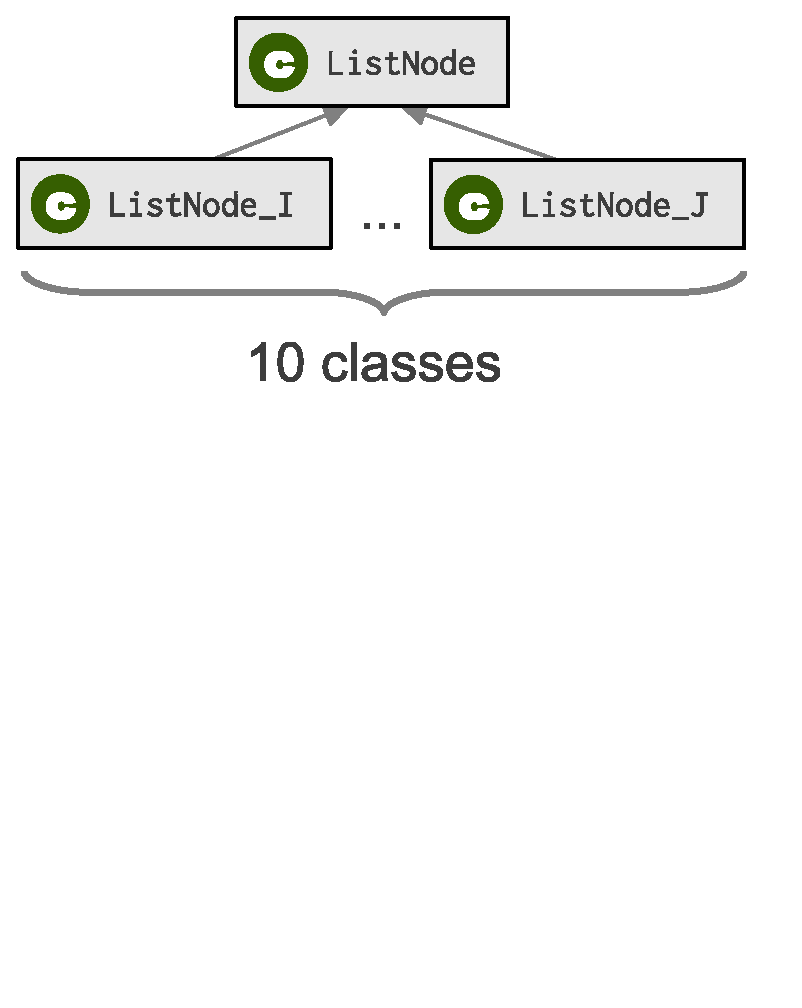
\includegraphics[width=0.5\textwidth]{diags/spec-diag.eps}
    \vspace{-16em}
    \caption[Class hierarchy generated by Specialization]{Class hierarchy generated by Specialization. The letters in class suffix represent the type they are specialized for: V-Scala Unit, Z-Boolean, B-Byte \ldots J-Long, L-AnyRef. The names are simplified throughout the chapter, and we avoid discussing the problem of name mangling, which was addressed in \cite{iuli-thesis}.}
    \label{mbox:fig-spec-diag}
\end{figure}

\topic{The} |ListNode| class has the generic |head| field, which needs to be specialized in order to avoid boxing. To this end, specialization will duplicate the class itself and adapt its fields for each primitive value type. Figure \ref{mbox:fig-spec-diag} shows the class hierarchy created: the parent class is the homogeneous translation of |ListNode|, which we also call generic class. The 10 subclasses are the specialized variants. They correspond to the 8 Java primitive types, |Unit| (which is Scala's object-oriented representation of |void|) and reference types\footnote{Technical note: For a single type parameter the reference variant will not be generated and the generic class will be used instead.}. Each of these specialized classes contains a |head| field of a primitive type, and inherits (or overrides) methods defined in the generic class. So far, specialization duplicated the class and adapted the fields, but in order to remove boxing the methods also need to be transformed heterogeneously.

\subsection{Method Specialization}
\label{mbox:subsec-spec-method}

\topic{In the specialized variants of} |ListNode|, the |contains| method needs to be duplicated and adapted to accept primitive values as arguments instead of their boxed representations. Since the |contains| method is already inherited from the generic class, it actually needs to be overridden. But it cannot be overridden, because its signature after the erasure \cite{java-erasure} transformation expects a reference type (|java.lang.Object|) and the specialized signature expects a primitive value. Therefore specialized methods need to be name-mangled, giving birth to new methods such as |contains_I| for |Int| and |contains_J| for |Long|.

\begin{figure}[t!]
    \vspace{-0.5em}
    \centering
    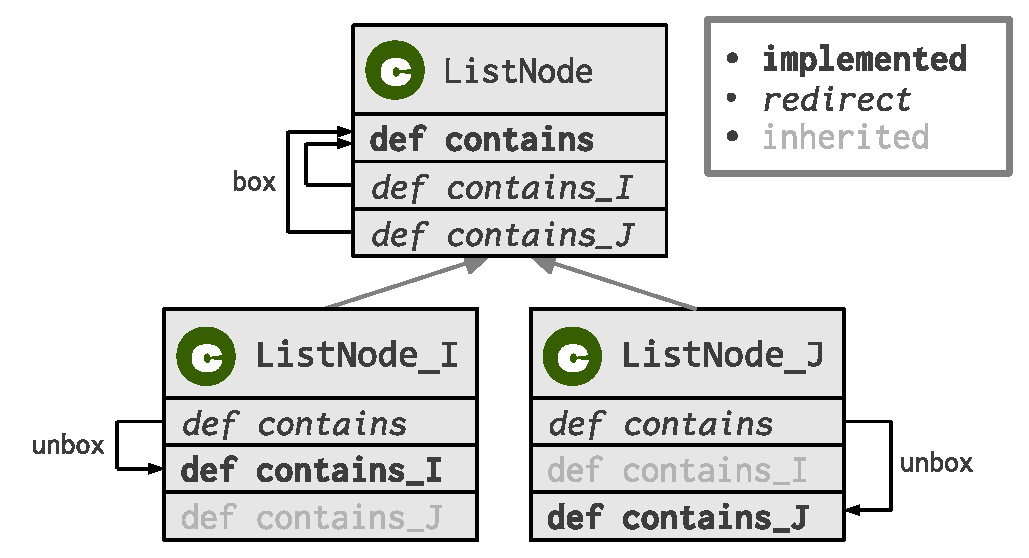
\includegraphics[width=0.65\textwidth]{diags/spec-methods.eps}
    \caption[Method overriding and redirection for ListNode and two variants]{Method overriding and redirection for ListNode and two of its specialized variants. Constructors and accessors are omitted from this diagram.}
    \label{mbox:fig-redirects}
    \vspace{-0.5em}
\end{figure}

\topic{The} |contains| method from the generic parent class will be inherited by all the specialized classes. But its code is generic and does not make use of primitive values, which is suboptimal. Therefore each specialized class overrides the generic |contains| and redirects it to the corresponding specialized variant, such as |contains_I| or |contains_J|. The redirection is done by unboxing the argument received by |contains| and calling the specialized method with the value type, as shown in Figure \ref{mbox:fig-redirects}. The same transformation is applied for accessors of specialized fields, such as |head| in the |ListNode| class. We defer the discussion of what happens to fields to Section \ref{mbox:subsec-spec-limits}.

\subsection{Opportunistic Tree Transformation}
\label{mbox:subsec-spec-rewiring}

\topic{The program code can only refer to generic classes and methods,} not their specialized variants. This happens because the specialization phase, which creates the variants, runs after the type checking phase. Thus the program is checked only against the generic classes and methods. But this does not mean specialization duplicates code in vain: aside from creating the variants, specialization also injects the specialized variants in the program code.

\topic{The last step in eliminating boxing is rewriting} the Scala abstract syntax tree (AST) to instantiate specialized classes and use specialized methods. We call this process rewiring. Rewiring works across separate compilation, as the specialization metadata is written in the generated bytecode. This makes is possible to use specialized code from libraries without carrying source code, like C++ does.

\topic{The instantiation rewiring injects specialized classes when the \textbf{new} keyword is used}. When the instantiated class has a more specific specialized variant for the given type arguments, the instantiation is rewired. Despite constructing a different class, the types in the AST are not adjusted to reflect this: In the example given below, although the instantiation is rewired to |new ListNode_I|, the type of |node1| remains |ListNode[Int]|. This makes specialization compatible: whether or not the instantiation is rewired, both the specialized class and the generic class are still subtypes of |ListNode[Int]|. Rewiring can only be done if the type arguments are statically known:

\begin{lstlisting-nobreak}
 // before rewiring:
 val node1: ListNode[Int] =
        new ListNode[Int](3, null)
 // after rewiring:
 val node1: ListNode[Int] =
        new ListNode_I(3, null)
 // not rewired if U is an abstract type or the
 // type parameter of an enclosing class/method
 val node2: ListNode[U] =
        new ListNode[U](u, null)
\end{lstlisting-nobreak}

\topic{The next step of rewiring changes inheritance relations} when parent classes have specialized variants that match the type arguments. This injects specialized variants of a class in the inheritance chain, making it possible to use unboxed values when extending a specialized class. This is yet another opportunistic transformation, since the inheritance relation is only rewritten if the type arguments are known statically, as shown by the following example:
%This is another opportunistic transformation, since the inheritance relation is only rewritten if the type parameter is known statically:

\begin{lstlisting-nobreak}
 // before rewiring:
 class IntNode(head: Int, tail: IntNode)
         extends ListNode[Int](head, tail)
 // after rewiring:
 class IntNode(head: Int, tail: IntNode)
         extends ListNode_I(head, tail)
 // not rewired, T not known statically:
 class MyNode[T](head: T, tail: MyNode[T])
         extends ListNode[T](head, tail)
\end{lstlisting-nobreak}

\topic{The two rewirings above inject specialized classes in the code.} Still, call sites point to the homogeneous methods, which use boxed values. The last rewiring addresses methods, which are rewritten depending on the type of their receiver. Any call site with a specialization-annotated receiver for which the type argument is statically known is rewritten to use specialized versions of the methods. In the first call site of the example below, the receiver is the specialization-annotated class |ListNode| and the type argument is statically known to be |Int|. Therefore the call to |contains| is rewired to the specialized |contains_I|:

\begin{lstlisting-nobreak}
 // before rewiring:
 (node1: ListNode[Int]).contains(3)
 // after rewiring:
 (node1: ListNode[Int]).contains_I(3)
 // not rewired if U is an abstract type or the
 // type parameter of an enclosing class/method
 (node2: ListNode[U]).contains(u)
\end{lstlisting-nobreak}

\subsection{Specialization Compatibility}
\label{mbox:subsec-spec-compatibility}

\topic{Since the rewiring process only takes place for statically known type arguments,} the generic class and its specialized subclasses may be mixed together. In the following snippet, the first branch of the |if| statement is rewired to create an instance of |ListNode_I| while the second branch calls the |node| method, whose type parameter |T| is not annotated for specialization, and thus creates the generic class |ListNode|. Therefore, the value |lst| (of static type |ListNode[Int]|) may be either an instance of |ListNode_I| or of |ListNode|, depending on the random condition:

\begin{lstlisting-nobreak}
 // new ListNode[T] not rewired to
 // ListNode_I since T is a type parameter
 def node[T](t: T) = new ListNode[T](t, null)

 val lst: ListNode[Int] =
   if (Random.nextInt().isEven)
     new ListNode[Int](1, null) // ListNode_I
   else
     node(2)                             // ListNode

 lst.contains(0) // rewired to contains_I
\end{lstlisting-nobreak}

\topic{Therefore,} calling a specialized method, |contains_I| in this case, can have as receivers both the generic class, |ListNode|, and the specialized one, |ListNode_I|. So both classes must implement the specialized method. To do so, in |ListNode|, |contains| will be implemented using generic code and |contains_I| will box the argument and call |contains|. In |ListNode_I|, |contains_I| will be implemented using primitive value types and |contains| will unbox and redirect. This can be generalized to multiple specialized variants, as can be seen in Figure \ref{mbox:fig-redirects}: The generic class at the top of the hierarchy contains all specialized variants of the |contains| method as redirects to the generic method. Then, each specialized variant of the class inherits from the generic class and overrides its corresponding specialized methods (such as |contains_I| for |ListNode_I|) with the heterogeneously transformed code and redirects the generic method to the specialized variant.

\topic{This shows the compatible nature of specialization:} in order to avoid boxing, both the call site and the receiver need to be rewired, which means the receiver needs to be specialized and the call site needs to know the type arguments statically or be part of code that will be specialized. But if either condition is not fulfilled, the code remains compatible by boxing, either at the call site itself or inside the redirecting method.

\topic{From the perspective of typing the abstract syntax trees}, compatibility is achieved because types are assigned before the specialization phase and are not modified later, so they refer to the generic class, even in the presence of rewiring. The first example in \S\ref{mbox:subsec-spec-rewiring} shows that despite rewiring the {\bf new} operator to create an instance of |ListNode_I|, the type of the |node1| value remains |ListNode[Int]|. Thus type-level compatibility is satisfied by |ListNode_I| being a subtype of |ListNode|, and the reverse subtyping is not necessary, as types never refer to |ListNode_I|\footnote{Except for the {\bf this} type and singleton types in the adapted code.}.

\subsection{Limitations of Specialization}
\label{mbox:subsec-spec-limits}

\topic{There are two limitations in specialization:} the bytecode explosion and the crippled specialized class inheritance. We will describe each problem and show how both can be addressed by the miniboxing encoding.

The specialization mechanism for generating variants is static: whenever the compiler encounters a class annotated for specialization, it generates all its variants up front and outputs bytecode for each of them. This is done to support separate compilation.

\topic{Theoretically, the specialized variant creation could be delayed} until the actual usage but this requires that the source files for specialized classes are available in all future compilation stages, exactly like in C++. This approach is undesirable from a user perspective, as it also requires encoding the original compilation flags and state, which can influence the generated code. Therefore the simplest, although bytecode-expensive solution was chosen: to generate specialized variants for all value types during compilation.

\topic{Fulfilling the bytecode compatibility requirements described before,} for $n$ type parameters and full specialization, means the generic class needs to implement $10^n$ methods, of which $10^n - 2$ are then inherited in the specialized subclasses and $2$ are overridden by each of the $10^n$ subclasses. This makes the bytecode size proportional to $10^n$. If the methods were not inherited but defined in each subclass, the bytecode size would be proportional to $10^{2n}$.

\topic{Still, the generic parent design choice affects inheritance between specialized classes.} Figure \ref{mbox:fig-spec-multi} shows an example where the design of specialization bumps into a multiple class inheritance, which is forbidden by Java. In this case, the children inherit from their generic parent, which is suboptimal, since the specialized variants of |MyList| cannot use the specialization in |ListNode|. Experienced Scala programmers might suggest that |MyNode| should be a trait, so it can be mixed in \cite{scalable-component-abstractions}. Indeed this solves the multiple inheritance problem, but creates bytecode proportional to $10^{2n}$, because the compiler desugars the trait into an interface, and each specialized |MyList_*| class has to implement the methods in that interface. Other more technical problems stem from this design choice too, but could be avoided by having an abstract parent class. For example, fields from the generic class are inherited by the specialized classes, therefore increasing their memory footprint. Constructors also require more complex code because instantiating a specialized class calls the constructor of its parent, the generic class, which needs to be prevented from running, such that side effecting operations in the original class' constructor are not executed twice.

\topic{All in all, at the heart of the bytecode explosion problem and thus the other} limitations of specialization, lies the large number of variants per type parameter: 10. For two type parameters, full specialization with correct inheritance creates $10^4$ times the bytecode. In practice this is not acceptable. Therefore a natural question to ask is how can we reduce the number of variants generated per type parameter? This is the question that inspired miniboxing.




\section{Data Representation Transformations}
\label{ildl:sec:drt}

As necessary background for our approach, we review data representation transformations and, in particular, the Late Data Layout transformation mechanism \cite{ldl}, which we later extend to our Ad hoc Data Representation Transformation.

Data can usually be represented in several ways, some more efficient and others more flexible. For example, integer numbers can use either the primitive (unboxed) value encoding, which is more efficient, or the object-based (boxed) encoding, which is more flexible. The boxed representation allows integers to act as the receivers of dynamically dispatched method calls, to be assigned to supertypes, such as |Number| or |Object| and to instantiate erased generics. However, the extra flexibility comes at a price: boxed integers are allocated on the heap so they need to be garbage-collected later and all their operations incur an indirection overhead. This leads to a tension between the two representations.

From a language perspective, there are two approaches to exposing the multiple representations of a type: either have a different type for each representation, as Java does, or fully hide the difference and present a single language-level type, as ML, Haskell and Scala do. Either way, the final low-level bytecode or assembly code needs to handle the two representations separately, since they correspond to very different entities: references and values.

Exposing a single high-level type in the language is more popular among programmers for its simplicity, but it places more responsibility on the compiler, which has to perform two additional steps: first, it needs to choose the data representation of each value; and second, it needs to introduce coercions that switch between representations where necessary. For example, since only boxed integers can instantiate generics, any unboxed integer going into a generic container, such as a list, needs to be \textem{coerced} to the boxed representation. This work is done in the compiler pipeline, in so-called data representation transformations.

The Late Data Layout (LDL) mechanism, presented next, is a powerful data
representation transformation facility for Scala.  It has three
properties that make it well-suited to be a substrate for our Ad hoc
Data Representation Transformation: selectivity, optimality and
consistency. However, LDL is neither programmer-driven, since the
data representation has to be known a priori and encoded in the
transformation, nor directly applicable to limited scopes inside a program,
so later sections will have to extend it.

\subsection{Late Data Layout}

The Late Data Layout (LDL) mechanism \cite{ldl} is the underlying transformation used in Scala to implement multi-parameter value class inlining and to specialize classes using the miniboxed encoding \cite{miniboxing}. It is a flexible and reliable mechanism, tested on thousands of lines of Scala code.

Using LDL, a language can expose high-level types (called high-level concepts in the LDL terminology), such as the integer type |Int| exposed by Scala, which can represent either a boxed or unboxed value in the low-level bytecode. In the following running example, we have values of types |Int| and |Any|. |Any| is the top of the Scala type system, and thus a supertype of |Int|:

\begin{lstlisting-nobreak}
val i: Int = 1
val j: Int = i
val k: Any = j
\end{lstlisting-nobreak}

Since Scala compiles down to Java bytecode, during compilation, the LDL-based primitive unboxing transformation bridges the gap between the high-level |Int| concept and its two representations: the unboxed |int| and the boxed |java.lang.Integer| representation. Along the way, it introduces the necessary coercions between these two representations. For example, the code above is translated to:\footnote{The translations shown throughout the paper are Scala compiler abstract syntax tree (AST) dumps, in different stages of the compilation. To facilitate reading, we pretty-print the ASTs using Scala syntax. Sometimes we have to introduce elements that are not part of the Scala syntax, such as |int|.}

\begin{lstlisting-nobreak}
val i: `int` = 1
val j: `int` = i
val k: Any = Integer.valueOf(j)
\end{lstlisting-nobreak}

The LDL mechanism transforms the data representation in three phases:
\inject{}, \coerce{} and \commit{}. Each of the phases is responsible
for a property of the transformation: \inject{} makes LDL
\emph{selective}, \coerce{} makes it \emph{optimal} and \commit{}
makes it \emph{consistent}. In our examples, we show the equivalent
source code for the program abstract syntax trees (ASTs) after each of
these phases.


\subsubsection*{The \Inject{} Phase}

The \inject{} phase is responsible for marking each symbol with its desired representation. In the case of primitive integer unboxing, the annotation is |@unboxed|, and it signals that the value should be stored in the unboxed |int| representation. As an optimization, instead of adding a |@boxed| annotation for the corresponding cases, symbols that are not marked are automatically considered boxed. Following the \inject{} phase, the previous example will be transformed to:


\begin{lstlisting-nobreak}
val i: `@unboxed` Int = 1 // Int can be unboxed
val j: `@unboxed` Int = i // Int can be unboxed
val k: Any = j                  // Any cannot be unboxed
\end{lstlisting-nobreak}


The \inject{} phase gives LDL a selective nature, al\-low\-ing it to mark
each individual symbol with its representation. For example, it would
have been equally correct if the marking rules decided that |j| should
be boxed, in which case it would not have been marked. One of
the properties of the LDL transformation is that boxed and unboxed
values are compatible in the \inject{} phase, so there are no coercions.


\subsubsection*{The \Coerce{} Phase}

The \coerce{} phase, as its name suggests, introduces coercions. This is done by changing the annotation semantics: annotated types become incompatible with their un-annotated counterparts. This change in the annotation semantics corresponds to introducing the different representations: each annotation corresponds to a representation, and representations are not compatible with each other. With this change, an assignment from one representation to another will lead to mismatching types. Therefore, by re-type-checking the tree, the \coerce{} phase can detect representation mismatches and can patch them using coercions. In the example, the last line contains such a mismatch:

\begin{lstlisting-nobreak}
val i: @unboxed Int = 1 // expected/found: @unboxed
val j: @unboxed Int = i // expected/found: @unboxed
val k: Any = `box`(j)             // mismatch => box
\end{lstlisting-nobreak}

The \coerce{} phase establishes the optimality property of the LDL transformation. The definition of optimality is quite involved, but we can easily show it using an example. Consider the following two integer definitions:

\begin{lstlisting-nobreak}
val c: Boolean = ...
val l1: @unboxed Int = if (c) i else j
val l2: @unboxed Int = `unbox`(if (c) `box`(i) else `box`(j))
\end{lstlisting-nobreak}

It is clear that the two definitions will always produce the same result. Yet, the first one is markedly better: it does not execute any coercions, compared to second definition, which executes two coercions regardless of the value of |c|. These subtle sub-optimalities can slow down program execution, increase the heap footprint and the bytecode size. The LDL paper \cite{ldl} makes the following intuition-based conjecture: ``in any given terminating execution trace through the transformed program, the number of coercions executed is minimal, for given sets of annotations introduced by the \inject{} phase and transformations performed in the \commit{} phase''. An initial formalization and proof is sketched in \cite{ldl-form}.

From our perspective, optimality means that once representations are chosen and annotated, the \coerce{} phase will not introduce any redundant coercions, so data will be seamlessly passed along with as few coercions as possible.


\subsubsection*{The \Commit{} Phase}

The \commit{} phase is responsible for introducing the actual representations. In the case of primitive unboxing, |@unboxed Int| is replaced by |int|, and |Int|, which is considered boxed, is replaced by |java.lang.Integer|. The |box| and |unbox| coercions are also replaced by the creation of objects and, respectively, by the extraction of the unboxed value:


\begin{lstlisting-nobreak}
val i: `int` = 1
val j: `int` = i
val k: Any = `Integer.valueOf`(j)
\end{lstlisting-nobreak}

The \commit{} phase is responsible for the consistency of the transformation. Since the program abstract syntax tree (AST) has been checked by the type-system extended with representation semantics, the \commit{} phase is guaranteed to correctly handle the value representations and to correctly coerce between them. This allows the \commit{} phase to be a very simple transformation over the program AST.

\subsection{Support For Object-Oriented Programming}
\label{ildl:sec:ldl:oo-patterns}

The LDL mechanism targets object-oriented programming languages, which pose unique challenges for data representation transformations. This section will describe the additional rules necessary in LDL to handle object-orientation.

\subsubsection*{Object-Oriented Patterns}

Aside from introducing coercions, data representation transformations must handle object-oriented patterns, such as method calls and subtyping. Not all representations can be used with these patterns. For example, it is not possible to call the |toString| method on the unboxed |int| representation:

\begin{lstlisting-nobreak}
val a: `@unboxed Int` = 1
println(a.toString)
\end{lstlisting-nobreak}

To handle dynamically dispatched method calls, LDL has a built-in rule: when a value acts as a method call receiver, it is coerced to the boxed representation, which, in this case, corresponds to the non-annotated representation. In our example, the |@unboxed Int| value is boxed during the \coerce{} phase, so it can act as the receiver of the |toString| method:

\begin{lstlisting-nobreak}
val a: @unboxed Int = 1
println(`box`(a).toString)
\end{lstlisting-nobreak}

To improve performance, the LDL mechanism also supports bypass methods, also known as
\emph{extension methods} in the literature. For example, if a static |bypass_toString| method is available for the unboxed |int| representation, there is no need to convert it before the method call:

\begin{lstlisting-nobreak}
val a: @unboxed Int = 1
println(`bypass_toString`(a))
\end{lstlisting-nobreak}

Subtyping is handled in a similar fashion, by requiring the boxed representation, which can be assigned to supertypes.

\subsubsection*{Support for Generics}

The Late Data Layout mechanism is agnostic to generics. This means that, depending on the transformation semantics and the implementation of generics, the mechanism can inject annotations in the type arguments or not. For example, if generics are erased, a list of integers will have type |List[Int]|, since values need to be boxed. If generics are unboxed and reified, the list type will be |List[@unboxed Int]|. The LDL paper \cite{ldl} shows examples of both cases: when annotations are propagated inside generics and when they are not. The LDL mechanism adapts seamlessly to either case.

Having seen the Late Data Layout mechanism at work for unboxing primitive types, we can now extend it to allow the more complex, programmer-driven, Ad hoc Data Representation Transformation.

\section{Ad hoc Data Representation Transformation}
\label{sec:ildl}

The Ad hoc Data Representation (ADR) transformation adds two new elements to existing data representation transformations: (1) it enables custom, programmer-defined alternative representations and (2) it allows the transformation to take place in limited scopes, ranging from expressions all the way to method and class definitions. This allows programmers to use locally optimal transformations that may be suboptimal or even incorrect for code outside the given scope.

Section \ref{sec:automating} showed how the ADR transformation is triggered by the |adrt| marker. The running example is reproduced below for quick reference:\footnote{In the following paragraphs, the |gcd| method is assumed to be always transformed, so we will skip the |ADRT| suffix, which was used in the Motivation section (\S\ref{sec:problem}) to mark the transformed version of the method.}

\begin{lstlisting-nobreak}
`adrt(IntPairComplexToLongComplex)` {
  def gcd(n1: (Int, Int), n2: (Int, Int)): (Int, Int)={
    val remainder = n1 % n2
    if (remainder.norm == 0) n2 else gcd(n2, remainder)
  }
}
\end{lstlisting-nobreak}

The following sections take a step by step approach to explaining how our technique allows programmers to define transformations and to use them in localized program scopes,  improving the performance of their programs in an automated and safe fashion.

\subsection{Transformation Description Objects}
\label{sec:ildl:custom}

The first step in performing an |adrt| transformation is defining the transformation description object. This object is required to extend a marker interface and to define the transformation through the |toRepr| and |toHigh| coercions:

\begin{lstlisting-nobreak}
object IntPairComplexToLongComplex
          extends TransformationDescription {
  // coercions:
  def `toRepr`(high: (Int, Int)): Long = ...
  def `toHigh`(repr: Long): (Int, Int) = ...
  // bypass methods:
  ...
}
\end{lstlisting-nobreak}

The coercions serve a double purpose: (1) the signatures match the high-level type, in this case |(Int, Int)| and indicate the corresponding representation type, |Long| and vice-versa and (2) the implementations are called in the transformed scope to encode and decode values as necessary.

Since the description objects can accommodate very different transformations, as shown in the Benchmarks section (\S\ref{sec:benchmarks}), we will not attempt to give a recipe for optimizing programs here. Each transformation should be devised by programmers based on runtime profiles and domain-specific knowledge of how data is processed inside the application. Instead, we will focus on the transformation facilities available to the description objects.

\subsubsection{Bypass Methods.} The description object can optionally include bypass methods, which correspond to the methods exposed by the high-level type, but instead operate on values encoded in the representation type. Bypass methods allow the transformation to avoid coercing receivers to the high-level type by rewriting dynamically dispatched calls to their corresponding statically-resolved bypass method calls, as shown in section \S\ref{sec:ldl:oo-patterns}. Method call rewriting in |adrt| scopes is more general, and we describe it   in section \S\ref{sec:ildl:method}.

\vspace{0.4em}
\subsubsection{Generic Transformations.} In our example, both the high-level and representation types are monomorphic (i.e., not generic). Still, in some cases, the ADR transformation is used to target collections regardless of the type of their elements. We analyzed multiple approaches to allowing genericity in the transformation description object and converged on allowing the coercions to be generic themselves. This approach has the merit of being concise and extending naturally to any type constructor arity:

\begin{lstlisting-nobreak}
  def toRepr[`T`](high: List[`T`]): LazyList[`T`] = ...
  def toHigh[`T`](repr: LazyList[`T`]): List[`T`] = ...
\end{lstlisting-nobreak}

Since the coercion signatures ``match'' the high-level type and return the corresponding representation type, a value of type |List[Int]| will be matched by the |adrt| transformation and subsequently encoded as a |LazyList[Int]|. This allows the |adrt| scopes to transform collections, containers and function representations. The benchmarks section (\S\ref{sec:benchmarks}) shows two examples of generic transformations.

\vspace{0.4em}
\subsubsection{Target Semantics.} It is worth noting that coercions defined in transformation objects must maintain the semantics of the high-level type. In particular, semantics such as mutability and referential identity must be preserved if the program relies on them. For example, correctly handling referential identity requires the coercions to return the exact same object (up to the reference) when interleaved:

\begin{lstlisting-nobreak}
assert(`toHigh(toRepr(x))` eq `x`) // referential equality
\end{lstlisting-nobreak}

These semantics prevent the coercions from simply copying the value of the object into the new representation.
For example, the referential equality condition above would be violated if the |toRepr| and |toHigh| methods would simply allocate new objects (which would get new references). Instead, the |toRepr| coercion would have to cache the original value so that, when decoding, the |toHigh| coercion could return the exact same object as originally given.

As expected, referential equality and mutability make transformations a lot more difficult. Luckily, in most use cases, the targets, such as library collections and containers, have value semantics: they are immutable, final and only use structural equality. Such high-level types can be targeted at will, since they can be reconstructed at any time without the program observing it. A desirable extension of our approach would be to statically check the compatibility of the high-level type with its coercions. This could prevent the programmer from incorrectly copying internally mutable objects inside the coercions.

The complete transformation description object for the complex number encoding is given in the Appendix.

\subsection{Transformation Scopes and Composability}
\label{sec:ildl:scoped}

Existing LDL-based data representation transformations, such as value class inlining and specialization, have fixed semantics and occur in separate compiler phases. Instead, the ADR transformation handles all scopes in the source code concurrently, each with its own high-level target, representation type, and coercions. This is a challenge, as handling the interactions between these concurrent scopes, some of which may even be nested, demands a disciplined treatment.

The key to handling all concurrent scopes correctly is shifting focus from the scopes themselves to the values they define. Since we are using the underlying LDL mechanism, we can track the encoding of each value in its type, using annotations. To keep track of the different transformations introduced by different scopes, we extend the LDL annotation system to reference the description object, essentially referencing the   transformation semantics with each individual value. We then leverage the type system and the signature persistence facilities to correctly transform all values, thus allowing scopes to safely and efficiently pass data among themselves, using the representation type---a property we refer to as composability.

We look at four instances of composability:

\vspace{0.3em}
\begin{itemize}
  \item allowing different scopes to communicate, despite using different representation types (high-level types coincide);
  \item isolating high-level types, barring unsound value leaks through the representation type;
  \item handling nested transformation description objects;
  \item passing values between high-level types in the encoded (representation) format;
\end{itemize}
\vspace{0.3em}

Although the four examples cover the most interesting corner cases of the transformation, the interested reader may consult the ``Scope Nesting'' page on the project wiki \cite{ildl-plugin-wiki}, which describes all cases of scope overlapping, collaboration and nesting. Furthermore, scope composition is tested with each commit, as part of the project's test suite.

\subsubsection{A high-level type can have different representations in different scopes.} This follows from the scoped nature of the ADR transformation, which allows programmers to use the most efficient data representation for each task. But it raises the question of whether values can be safely passed across scopes that use different representations:

\begin{lstlisting-nobreak}
adrt(IntPairToLong)   { var x = (3, 5) }
adrt(IntPairToDouble) { val y = (2, 6); `x = y` }
\end{lstlisting-nobreak}

At a high level, the code is correct: the variable |x| is set to the value of |y|, both of them having high-level type |(Int, Int)|. However, being in different scopes, these two values will be encoded differently, |x| as a long integer and |y| as a double-precision floating point number. In this situation, how will the assignment |x = y| be translated? Let us look at the transformation step by step.

After parsing, the scope is inlined and the program is type-checked against the high-level types. Aside from checking the high-level types, the type checker also resolves implicits and infers all missing type annotations. While type-checking, the description objects are stored as invisible abstract syntax tree attachments (described in \S\ref{sec:impl}):

\begin{lstlisting-nobreak}
var x: (Int, Int) = (3, 5) /* att: IntPairToLong */
val y: (Int, Int) = (2, 6) /* att: IntPairToDouble */
`x = y`
\end{lstlisting-nobreak}

Then, during the \inject{} phase, each value or method definition that matches the description object's high-level type is annotated with the |@repr| annotation, parameterized on the transformation description object:

\begin{lstlisting-nobreak}
var x: `@repr(IntPairToLong)` (Int, Int) = (3, 5)
val y: `@repr(IntPairToDouble)` (Int, Int) = (2, 6)
x = y
\end{lstlisting-nobreak}

The |@repr| annotation is only attached if the value's type matches the high-level type in the description object. Therefore, programmers are free to define values of any type in the scope, but only those values whose type matches the transformation description object's target will be annotated.

Based on the annotated types, the \coerce{} phase notices the mismatching transformation description objects in the last line: the left-hand side is on its way to be converted to a long integer (based on the description object |IntPairToLong|) while the right-hand side will become a floating point expression (based on the description object |IntPairToDouble|). However, both description objects have the same high-level type, the integer pair, which can be used as a middle ground in the conversion:

\begin{lstlisting-nobreak}
var x: @repr(IntPairToLong) (Int, Int) = `toRepr`(IntPairToLong, (3, 5))
val y: @repr(IntPairToDouble) (Int, Int) = `toRepr`(IntPairToDouble, (2, 6))
x = `toRepr`(IntPairToLong, `toHigh`(IntPairToDouble, y))
\end{lstlisting-nobreak}

Finally, the \commit{} phase transforms the example to:

\begin{lstlisting-nobreak}
var x: `Long` = IntPairToLong.toRepr((3, 5))
val y: `Double` = IntPairToDouble.toRepr((2, 6))
x = IntPairToLong.toRepr(IntPairToDouble.toHigh(y))
\end{lstlisting-nobreak}

In the end, the value |x| is converted from a double to a pair of integers, which is subsequently converted to a long integer. This shows the disciplined way in which different |adrt| scopes compose, allowing values to flow across different representations, from one scope to another. Similarly to the LDL transformation, the mechanism aims to employ a minimal number of conversions.

\vspace{0.65em}

\subsubsection{Different transformation scopes can be safely nested} and the high-level types are correctly isolated:

\begin{lstlisting-nobreak}
adrt(`FloatPairAsLong`) {
  adrt(`IntPairAsLong`) {
    val x: `(Float, Float)` = (1f, 0f)
    var y: `(Int, Int)` = (0, 1)
    // y = x
    // y = 123.toLong
  }
}
\end{lstlisting-nobreak}

Values of the high-level types in the inner scope are independently annotated and are transformed accordingly. Since both the integer and the float pairs are encoded as long integers, a natural question to ask is whether values can leak between the two high-level types, for example, by un-commenting the last two lines of the inner scope. This would open the door to incorrectly interpreting an encoded value as a different high-level type, thus introducing unsoundness.

The answer is no: the code is first type-checked against the high-level types even before the \inject{} transformation has a chance to annotate it. This prohibits direct transfers between the high-level types and their representations. Thus, the unsound assignments will be rejected, informing the programmer that the types do not match. This is a non-obvious benefit of using the ADR transformation instead of manually refactoring the code and using implicit conversions, which, in some cases, would allow such unsound assignments.

\vspace{-0.3em}

\subsubsection{Handling nested transformation description objects} is another important property of composition:

\begin{lstlisting-nobreak}
adrt(`PairAsMyPair`) {            // (Int,Int) -> MyPair[Int,Int]
  adrt(`IntPairAsLong`) { // (Int,Int) -> Long
    val x: `(Int, Int)` = (2, 3)
  }
  println(x.toString)
}
\end{lstlisting-nobreak}

In the code above, the type of |x| matches both transformation description objects, so it could be transformed to both representation types |MyPair[Int, Int]| and |Long|. However, during the \inject{} phase, if a value is matched by several nested |adrt| scopes, this can be reported to the programmer either as an error or, depending on the implementation, as a warning, followed by choosing one of the transformation description objects for the value (our current solution):

\begin{lstlisting-nobreak}
console:9:  warning: Several adrt scopes can be applied to value x. Picking the innermost one: `IntPairAsLong`
val x: `(Int, Int)` = (2, 3)
          ^
\end{lstlisting-nobreak}

Furthermore, since the \inject{} phase annotates value |x| with the chosen transformation, there will be no confusion on the next line, where |x| has to be converted back to the high-level type to receive the |toString| method call, despite the fact that the |adrt| scope surrounding the instruction uses a different transformation description object.

A different case of nested transformation description objects is what we call ``cascading'' scopes:

\begin{lstlisting-nobreak}
adrt(`TtoU`) {             // T -> U
  adrt(`UtoV`) {           // U -> V
    val t: `T` = ???       // T -> U -> V (?)
  }
}
\end{lstlisting-nobreak}

It may seem natural that the value |t| will be transformed to use the |V| representation type: first, converting from |T| to |U| and then from |U| to |V|. Unfortunately, the underlying mechanism, Late Data Layout \cite{ldl}, only allows values to undergo one representation change in the \coerce{} phase. Thus, to enable cascading scopes, we would have to either run the \coerce{} phase until a fixpoint or extend both the theory and the implementation to handle multiple conversions in a single run, neither of which is a straightforward extension.
Therefore, in the current approach, we disallow cascading scopes:

\begin{lstlisting-nobreak}
cascading.scala:25:  warning: Although you may expect value t to use the representation type U, by virtue of nesting the transformation description objects (TtoU,UtoV), "cascading" scopes are not supported:
val t: `T` = ???
         ^
\end{lstlisting-nobreak}

Instead, the value |t| undergoes a single ADR transformation, to the representation type |V|. By disallowing ``cascading'' scopes we also protect against cyclic scopes, such as |TtoU| nested inside |UtoT|, which could cause infinite loops.

\vspace{-0.2em}
\subsubsection{Prohibiting access to the representation type inside the transformation scope is limiting.} For example, a per\-for\-mance-conscious programmer might want to transform the high-level integer pair into a floating-point pair without allocating heap objects. Since the programmer does not have direct access to the representation, it looks like the only solution is to decode the integer pair into a heap object, convert it to a floating-point pair and encode it back to the long integer.

There is a better solution. As we will later see, the programmer can use bypass methods to ``serialize'' the integer pair into a long integer and ``de-serialize'' it into a floating-point pair. Yet, this requires a principled change in the transformation description object. This is the price to pay for a safe and automated representation transformation.

To recap: focusing on individual values and storing the transformation semantics in the annotated type allows us to correctly handle values flowing across scopes, a property we call scope composition. Although we focused on values, method parameters and return types are annotated in exactly the same way. The next part extends scope composition across separate compilation.

\vspace{-0.5em}
\subsection{Separate Compilation}
\label{sec:ildl:separate-compilation}
\vspace{-0.3em}

Annotating the high-level type with the transformation semantics allows different |adrt| scopes to seamlessly pass encoded values. To reason about composing scopes across different compilation runs, let us assume we have already compiled the |gcd| method in the motivating example:

\begin{lstlisting-nobreak}
`adrt(IntPairComplexToLongComplex)` {
  def gcd(n1: (Int,Int), n2: (Int,Int)): (Int,Int) =...
}
\end{lstlisting-nobreak}

After the \inject{} phase, the signature for method |gcd| is:

\begin{lstlisting-nobreak}
def gcd(
    n1: `@repr(IntPairComplexToLongComplex)` (Int, Int),
    n2: `@repr(IntPairComplexToLongComplex)` (Int, Int)
  ): `@repr(IntPairComplexToLongComplex)` (Int, Int) = ...
\end{lstlisting-nobreak}

And, after the \commit{} phase executed, the bytecode signature for method |gcd| is:

\begin{lstlisting-nobreak}
def gcd(n1: `long`, n2: `long`): `long` = ...
\end{lstlisting-nobreak}

When compiling source code that refers to existing low-level code, such as object code or bytecode compiled in a previous run, compilers need to load the signature of each symbol. For C and C++ this is done by parsing header files while for Java and Scala, it is done by reading the source-level signature from the bytecode metadata. However, not being aware of the ADR transformation of method |gcd|, a separate compilation could assume it accepts two pairs of integers as input. Yet, in the bytecode, the |gcd| method accepts long integers and cannot handle pairs of integers.

The simplest solution is to create two versions for each transformed method: the transformed method itself and a bridge, which corresponds to the high-level signature. The bridge method would accept pairs of integers and encode them as longs before calling the transformed version of the |gcd| method. It would also decode the result of |gcd| back to a pair of integers. This approach allows calling |gcd| from separately compiled files without being aware of the transformation. Still, we can do better.

\vspace{-0.45em}
\subsubsection{Persisting transformation annotations.} Let us assume we want to call the |gcd| method from a scope transformed using the same transformation description object as we used when compiling |gcd|, but in a different compilation run:

\begin{lstlisting-nobreak}
`adrt(IntPairComplexToLongComplex)` {
  val n1: (Int, Int) = ...
  val n2: (Int, Int) = ...
  val res: (Int, Int) = gcd(n1, n2)
}
\end{lstlisting-nobreak}

In this case, would it make sense to call the bridge method? The values |n1| and |n2| are already encoded, so they would have to be decoded before calling the bridge method, which would then encode them back. This is suboptimal.

Instead, we want the |adrt| scopes to compose across separate compilation, allowing the call to go through in the encoded format.  This is achieved by persisting the transformation information in the generated bytecode, but we have to do so without making ADR transformations a first-class concept. The approach we took is to persist the injected annotations, including the reference to the transformation description object. These become part of the signature of |gcd|:

\begin{lstlisting-nobreak}
// loaded signature (description object abbreviated):
def gcd(n1: @repr(.) (Int, Int), n2: @repr(.) (Int, Int)): @repr(.) (Int, Int)
\end{lstlisting-nobreak}

The annotations are loaded just before the \inject{} phase, which transforms our code to:

\begin{lstlisting-nobreak}
val n1: `@repr(.)` (Int, Int) = ...
val n2: `@repr(.)` (Int, Int) = ...
val res: `@repr(.)` (Int, Int) = gcd(n1, n2)
\end{lstlisting-nobreak}

With the complete signature for |gcd|, the \coerce{} phase does not introduce any coercions, since the arguments to method |gcd| use the same encoding as the method parameters did in the previous compilation run. This allows |adrt| scopes to seamlessly compose even across separate compilations. After the \commit{} phase, the scope is compiled to:

\begin{lstlisting-nobreak}
val n1: `Long` = ...
val n2: `Long` = ...
val res: `Long` = gcd(n1, n2) // no coercions!!!
\end{lstlisting-nobreak}

\vspace{-0.45em}
\subsubsection{Making bridge methods redundant.} Persisting transformation information in the high-level signatures allows us to skip creating bridges. For example:

\vspace{-0.2em}
\begin{lstlisting}
val res: (Int, Int) = gcd((55, 2), (17, 13))
\end{lstlisting}

Since the signature for method |gcd| references the transformation description object, the \coerce{} phase knows exactly which coercions are necessary:

\begin{lstlisting-nobreak}
val res: (Int, Int) = `toHigh`(...,
  gcd(`toRepr`(..., (55, 2)), `toRepr`(..., (17, 13))))
\end{lstlisting-nobreak}

Generally, persisting references to the description objects in each value's signature allows efficient scope composition across separate compilation runs.

\vspace{-0.5em}
\subsection{Optimizing Method Invocations}
\label{sec:ildl:method}
\vspace{-0.2em}

When choosing a generic container, such as a pair or a list, programmers are usually motivated by the natural syntax and the flexible interface, which allows them to quickly achieve their goal by invoking the container's many convenience methods. The presentation so far focused on optimizing the data representation, but to obtain peak performance, the method invocations need to be transformed as well:

\begin{lstlisting-nobreak}
adrt(`IntPairComplexToLongComplex`) {
  val n = (0, 1)
  println(n.toString)
}
\end{lstlisting-nobreak}

When handling method calls on an encoded receiver, the default LDL behavior is very conservative: it decodes the value back to its high-level type, which exposes the original method and generates a dynamically-dispatched call (\S\ref{sec:ldl:oo-patterns}):

\begin{lstlisting-nobreak}
val n: Long = ...
println(`IntPairComplexToLongComplex.toHigh(n)`.toString)
\end{lstlisting-nobreak}

The price to pay is decoding the value into the high-level type, which usually leads to heap allocations and can introduce overheads. If a corresponding bypass method is available, the LDL transformation can use it:

\begin{lstlisting-nobreak}
val n: Long = ...
println(IntPairComplexToLongComplex.`bypass_toString`(n))
\end{lstlisting-nobreak}

The bypass method can operate directly on the encoded version of the integer pair, avoiding a heap allocation. In practice, when the receiver of a method call is annotated, our modified LDL transformation looks up the |bypass_toString| method in the transformation description object, and, if none is found, warns the programmer and proceeds with decoding the receiver and generating the dynamically-dispatched call.

\vspace{-0.2em}
\subsubsection{Methods added via implicit conversions} and other enrichment techniques, such as extension methods or type classes, add another layer or complexity, only handled in the ADR transformation. For example, we can see the multiplication operator |*|, added via an implicit conversion (we will further analyze the interaction with implicit conversions in \S\ref{sec:ildl:language-implicit-conversions}):

\begin{lstlisting-nobreak}
adrt(`IntPairComplexToLongComplex`) {
  val n1 = (0, 1)
  val n2 = n1 * n1
}
\end{lstlisting-nobreak}

Type-checking the program produces an explicit call for the implicit conversion that introduces the |*| operator:

\vspace{-0.5em}
\begin{lstlisting}
val n1: (Int, Int) = (0, 1)
val n2: (Int, Int) = `intPairAsComplex(n1)` * n1
\end{lstlisting}

This is a costly pattern, requiring |n1| to be decoded into a pair and passed to the |intPairAsComplex| method, which itself creates a wrapper object that exposes the |*| operator. To optimize this pattern, the ADR transformation looks for a bypass method in the transformation description object that corresponds to a mangled name combining the implicit method name and the operator. For simplicity, if we assume the name is |implicit_*| and the bypass exists in the |IntPairComplexToLongComplex| object, the \coerce{} phase transforms the code to:

\begin{lstlisting-nobreak}
val n1: Long = toRepr((0,1))
val n2: Long = IntPair...Complex.`implicit_*(n1, n1)`
\end{lstlisting-nobreak}

This allows the call to the |*| operator to be transformed into a bypass call, avoiding heap object creation, and thus significantly improving the performance and heap footprint.

\vspace{-0.4em}
\subsubsection{Bypass methods.} Both normal and implicit bypass methods defined in the transformation description object need to correspond to the original method they are replacing and:

\begin{itemize}
\item Add a first parameter corresponding to the receiver;
\item Have the rest of the parameters match the origin method;
\item Freely choose parameters to be encoded or decoded.
\end{itemize}

Therefore, during the \coerce{} phase, which introduces bypass method calls, the |implicit_*| has the signature:

\begin{lstlisting-nobreak}
def implicit_*(recv: `@repr(...) (Int, Int)`,  n2: `@repr(...) (Int, Int)`): `@repr(...) (Int, Int)`
\end{lstlisting-nobreak}

Since the programmer defining the description object is free to choose any encoding for the bypass arguments, the following (suboptimal) signature would be equally accepted:

\begin{lstlisting-nobreak}
def implicit_*(recv:`(Int,Int)`, n2:`(Int,Int)`):`(Int,Int)`
\end{lstlisting-nobreak}

With the second signature, despite calling a bypass method, the arguments still have to be coerced, since the high-level type |(Int, Int)| is expected.

It is interesting to notice that representation-agnostic method rewriting relies on two previous design choices: \\
(1) shifting focus from scopes to individual values and \\
(2) carrying the entire transformation semantics in the signature of each encoded value.
Yet, there is still a snag.

\vspace{-0.4em}
\subsubsection{Constructors} create heap objects before they can be encoded in the representation type. In our example, the first line runs the pair (|Tuple2|) constructor, which creates a heap object, and then converts it to the |Long| representation:

\begin{lstlisting-nobreak}
// In Scala, (0,1) is a shorthand for new Tuple2(0,1):
val n1: Long = toRepr(`(0,1)`)
val n2: Long = IntPair...Complex.implicit_*(n1, n1)
\end{lstlisting-nobreak}

Instead of allocating the |Tuple2| object, the ADR transformation can intercept and rewrite constructor invocations into constructor bypass methods:

\begin{lstlisting-nobreak}
val n1: Long = `IntPair...Complex.ctor_Tuple2(0, 1)`
val n2: Long = IntPair...Complex.implicit_*(n1, n1)
\end{lstlisting-nobreak}

Notice that the integers are now passed as arguments to the constructor bypass method |ctor_Tuple2|, by value. This completes this scope's transformation, allowing it to execute without allocating any heap object at all.

\subsection{Interaction with Other Language Features}
\label{sec:ildl:language-features}

This section presents the interaction between the ADR transformation and object-oriented inheritance, generics and implicit conversions, explaining the additional steps that are taken to ensure correct program transformation.

\subsubsection{Dynamic Dispatch and Overriding}
\label{sec:ildl:language-overriding}
are an integral part of the object-oriented programming model, allowing objects to encapsulate code. The main approach to evolving this encapsulated code is extending the class and overriding its methods. However, changing the data representation can lead to situations where source-level overriding methods are no longer overriding in the low-level bytecode:

\begin{lstlisting-nobreak}
trait X {
  def identity(i: (Int, Int)): (Int, Int) = i
}
`adrt(IntPairAsLong)` {
  class Y(t: (Int, Int)) extends X {
    override def identity(i: (Int, Int)) = t
  }
}
\end{lstlisting-nobreak}

After the ADR transformation, the |identity| method in class |Y| no longer overrides method |identity| in trait |X|, since its signature expects a long integer instead of a pair of integers. To address this problem, we extend the Late Data Layout mechanism by introducing a new \bridge{} phase, which runs just before \coerce{} and inserts bridge methods to enable correct overriding. After the \inject{} phase, the code corresponding to class |Y| is:

\begin{lstlisting-nobreak}
class Y(t: `@repr(...)` (Int, Int)) extends X {
  override def identity(i: `@repr(...)` (Int, Int)) = t
}
\end{lstlisting-nobreak}

The \bridge{} phase inserts the methods necessary to allow correct overriding (return types are omitted):

\begin{lstlisting-nobreak}
class Y(t: `@repr(...)` (Int, Int)) extends X {
  def identity(i: `@repr(...)` (Int, Int)) = t
  @bridge // overrides method identity from class X:
  override def identity(i: `(Int, Int)`) = identity(i)
}
\end{lstlisting-nobreak}

The \coerce{} and \commit{} phases then transform class |Y| as before, resulting in a class with two methods, one containing the optimized code and another that overrides the method from class |X|, marked as |@bridge|:

\begin{lstlisting-nobreak}
class Y(t: `Long`) extends X {
  def identity(i: `Long`): `Long` = t
  @bridge override def identity(i: `(Int, Int)`) = ...
}
\end{lstlisting-nobreak}

If we now try to extend class |Y| in another |adrt| scope with the same transformation description object, overriding will take place correctly: the new class will define both the transformed method and the bridge, overriding both methods above. However, a more interesting case occurs when extending class |Y| from a scope with a different description:

\begin{lstlisting-nobreak}
adrt(`IntPairAsDouble`) { // != IntPairAsLong
  class Z extends Y(...) {
    override def identity(i: (Int, Int)): (Int, Int) = i
  }
}
\end{lstlisting-nobreak}

The ensuing \bridge{} phase generates 2 bridge methods:

\begin{lstlisting-nobreak}
class Z extends Y(...) {
  def identity(i: `Double`): `Double` = i
  @bridge override def identity(i: `(Int, Int)`) = ...
  @bridge override def identity(i: `Long`): `Long` = ...
}
\end{lstlisting-nobreak}

Although the resulting object layout is consistent, the |@bridge| methods have to transform between the representations, which makes them less efficient. This is even more problematic when up-casting class |Z| to |Y| and invoking |identity|, as the bridge method goes through the high-level type to convert the long integer to a double. In such cases the \bridge{} phase issues warnings to notify the programmer of a possible slowdown caused by the coercions.

\subsubsection{Dynamic and Native Code.} Thanks to the \bridge{} phase, class |Z| conforms to the trait (interface) |X|, thus, any call going through the interface will execute as expected, albeit, in this case, less efficiently. This allows dynamically loaded code to work correctly:

\label{sec:ildl:language-dynamically-loaded-code}

\begin{lstlisting-nobreak}
Class.forName("Z").newInstance() match {
  case x: X[_] => x.identity((3, 4))
  case _ => throw new Exception("...")
}
\end{lstlisting-nobreak}

We have not tested the Java Native Interface (JNI) with ADR transformations, but expect the object layout assumptions in the C code to be invalidated. However, method calls should still occur as expected.

\subsubsection{Generics.}
\label{sec:ildl:language-generics}
Another question that arises when performing ad hoc programmer-driven transformations is how to transform the data representation in generic containers. Should the ADR transformation be allowed to change the data representation stored in a |List|? We can use an example:

\begin{lstlisting-nobreak}
def use1(list: List[(Int, Int)]): Unit = ...
adrt(IntPairAsLong) {
  def use2(list: List[(Int, Int)]): Unit = `use1(list)`
}
\end{lstlisting-nobreak}

In the specific case of the Scala immutable list, it would be possible to convert the |list| parameter of |use2| from type |List[Long]| to |List[(Int, Int)]| before calling |use1|. This can be done by mapping over the list and transforming the representation of each element. However, this domain-specific knowledge of how to transform the collection only applies to the immutable list in the standard library, and not to other generic classes that may occur in practice. Furthermore, there is an entire class of containers for which this approach is incorrect: mutable containers. An invariant of mutable containers is that any elements changed will be visible to all the code that holds a reference to the container. Duplicating the container itself and its elements (stored with a different representation) breaks this invariant: changes to one copy of the mutable container are not visible to its other copies. This is similar to the mutability restriction in \S\ref{sec:ildl:custom}.

The approach we follow in the ADR transformation is to preserve the high-level type inside generics. Thus, our example after the \commit{} phase will be:

\begin{lstlisting-nobreak}
def use1(list: List[(Int, Int)]): Unit = ...
def use2(list: List[(Int, Int)]): Unit = `use1(list)`
\end{lstlisting-nobreak}

However, this does not prevent a programmer from defining another transformation description object that targets |List[(Int, Int)]| and replaces it by |List[Long]|:

\begin{lstlisting-nobreak}
adrt(`ListOfIntPairAsListOfLong`) {
  def use3(list: List[(Int, Int)]): Unit = use1(list)
}
\end{lstlisting-nobreak}

In this second example, following the \commit{} phase, the |List[(Int, Int)]| is indeed transformed to |List[Long]|:

\begin{lstlisting-nobreak}
def use3(list: `List[Long]`): Unit = use1(`toHigh`(list))
\end{lstlisting-nobreak}

To summarize, |adrt| scopes are capable of targeting:

\vspace{0.3em}
\begin{itemize}
\item generic types, such as |List[T]| for any |T|;
\item instantiated generic types, such as |List[(Int, Int)]|;
\item monomorphic types, such as |(Int,Int)|, outside generics
\end{itemize}
\vspace{0.3em}

\noindent
Using these three cases and scope composition, programmers can conveniently target any type in their program.

\subsubsection{Implicit conversions}
\label{sec:ildl:language-implicit-conversions}
interact in two ways with |adrt| scopes:

\vspace{0.3em}
\noindent
\textem{Extending the object functionality} through implicit conversions, extension methods, or type classes must be taken into account by the method call rewriting in the \coerce{} phase. The handling of all three means of adding object functionality is similar, since, in all three cases, the call to the new method needs to be intercepted and redirected. Depending on the exact means, the mangled name for the bypass method will be different, but the mechanism and signature transformation rules remain the same (\S\ref{sec:ildl:method}).

\vspace{0.3em}
\noindent
\textem{Offering an alternative transformation mechanism}. Despite the apparent similarity, implicit conversions are not powerful enough to replace the ADRT mechanism. For example, assuming the presence of implicit methods to coerce integer pairs to longs and back, we can try to transform:

\begin{lstlisting-nobreak}
val n: (Int, Int) = (1, 0)
val a: Any = n
println(a)
\end{lstlisting-nobreak}

\noindent
To trigger the transformation, we update the type of |n| to |Long| in the source code and wait for the implicit conversions to do their work:

\begin{lstlisting-nobreak}
val n: `Long` = (1, 0) // triggers implicit conversion
val a: Any = n              // does not trigger the reverse
println(a)
\end{lstlisting-nobreak}

This resulting code breaks semantics because no coercion is applied to |a|, since |Long| is a subtype of |Any|. In turn, the output becomes |4294967296| instead of |(1, 0)|. As we saw in \S\ref{sec:drt}, the missing coercion is correctly inserted when annotations track the value representation, since annotations are orthogonal to the host language type system.

With this, we presented the Ad hoc Data Representation Transformation mechanism and how it interacts with other language features to guarantee transformation correctness. The next section describes the architecture and implementation of our Scala compiler plugin. \iv{Hey, is this thing on?}

\section{Implementation}
\label{sec:impl}

We implemented the ADR transformation as a Scala compiler plugin \cite{ildl-plugin}, by extending the open-source multi-stage programming transformation provided with the LDL \cite{ldl} artifact, available at \cite{ldl-staging-plugin}. In this section we describe the technical aspects of our implementation that are not directly related to the transformation itself, but to providing a good programmer experience. Readers should also refer to the paper Appendix for an end-to-end example of the transformation phases. Additionally, the paper is accompanied by an artifact which can be used to explore the transformation.


\noindent \textbf{The} |adrt| \textbf{scope} acts as the trigger for the ADR transformation.
We treat it as a special keyword that we transform immediately after parsing, in the \postparser{} phase.
To show this, we follow a program through the compilation stages:

\begin{lstlisting-nobreak}
def foo: (Int, Int) = {
  adrt(IntPairToLong) {
    val n: (Int, Int) = (2, 4)
  }
  n
}
\end{lstlisting-nobreak}

\noindent
Immediately after the source is parsed, the \postparser{} phase transforms the |adrt| scopes in three steps:


\begin{itemize}
\item it attaches a unique id to each |adrt| scope;
\item it records and clears the block enclosed by the |adrt| scope
\item it inlines the recorded code immediately after the now-empty
|adrt| scope and, in the process, it marks the value and method definitions
by the |adrt| scope's unique id (or by multiple ids, if |adrt| scopes are nested).
\end{itemize}


\noindent Following the \postparser{} phase, the code is:

\begin{lstlisting-nobreak}
def foo: (Int, Int) = {
  /* id: 100 */ adrt(IntPairToLong) {}
  /* id: 100 */ val n: (Int, Int) = (2, 4)
  n
}
\end{lstlisting-nobreak}

This code is ready for type-checking: the definition of |n| is located in the same block as its use, making the scope correct. During the type-checking process, the |IntPairToLong| object is resolved to a symbol, missing type annotations are inferred and implicit conversions are introduced explicitly in the tree. After type-checking and pattern matching expansion, the \inject{} phase traverses the tree and:


\begin{itemize}
\item for every |adrt| scope it records the id and description object, before removing it from the abstract syntax tree;
\item for value and method definitions, if the type matches one or more transformations, it adds the |@repr| annotation.
\end{itemize}


\noindent Following the \inject{} phase, the code for our example is:

\begin{lstlisting-nobreak}
def foo: (Int, Int) = {
  val n: `@repr(IntPairToLong)` (Int, Int) = (2, 4)
  n
}
\end{lstlisting-nobreak}

\noindent
After the \inject{} phase, the annotated signatures are persisted, allowing the scope composition to work across separate compilation.
Later, the \bridge{}, \coerce{} and \commit{} phases proceed as described in \S\ref{sec:drt} and \S\ref{sec:ildl}.

\subsubsection*{The transformation description objects} extend the marker trait |TransformationDescription|. Although the marker trait is empty, the description object needs to define at least the |toHigh| and |toRepr| coercions, which may be generic, as shown in \S\ref{sec:ildl:custom}. The programmer is then free to add bypass methods, in order to avoid decoding the representation type for the purpose of dynamically dispatching method calls. To aid the programmer in adding bypass methods, the \coerce{} phase warns whenever it does not find a suitable bypass method, indicating both the expected name and the expected method signature. \iv{Help, I'm trapped here!}

Here we encountered a bootstrapping problem: although bypass methods handle the representation type, during the \coerce{} phase, their signatures are expected to take parameters of the annotated high-level type, in order to allow redirecting method calls. To work around this problem, we added the |@high| annotation, which acts as an anti-|@repr| and marks the representation types:

\begin{lstlisting-nobreak}
object IntPairToLong extends TransformationDescription{
  ...
  // source-level signature (type-checking the body):
  def bypass_toString(repr: `@high` Long): String = ...
  // signature during coerce (allows rewriting calls):
  //   def bypass_toString(repr: @repr(...) (Int, Int))
  // signature after commit (bytecode signature):
  //   def bypass_toString(repr: Long)
}
\end{lstlisting-nobreak}

This mechanism allows programmers to both define and use the transformation description objects in the same compilation run---an obvious benefit over full macro-based metaprogramming in Scala \cite{eugene-macros}. This reflects our design decision to only allow the description object to drive the transformation through its members and types, without running code that manipulates the AST. \iv{So stop complaining!}

Another advantage we get for free, thanks to referencing the transformation description object in the type annotation, is an explicit dependency between all transformed values and their description objects. This allows the Scala incremental compiler to automatically recompile all scopes when the description object in their |adrt| marker has changed.



\paragraph*{Compiler Entry Points.}

In many of the descriptions so far we have implicitly assumed the Scala compiler features. To ease other compiler developers in porting this approach, we highlight the exact Scala compiler features that we use:


\begin{itemize}
  \item The type checker is available at all times during compilation;
  \item We can change/see a symbol's signature at any phase;
  \item The compiler supports type annotations and external annotation checkers;
  \item The compiler support AST attachments;
  \item The compiler offers expected type propagation during type checking (In Scala, this is part of the local type inference.)
\end{itemize}


This concludes the section, which explained how we solved the main technical problems in the ADR Transformation and how this impacted the compilation pipeline. We now continue with our experimental evaluation.

\section{Benchmarks}
\label{sec:benchmarks}
\label{sec:benchmarks:ad-hoc}

This section evaluates the experimental benefits of ADR transformations in targeted micro-benchmarks and in
the setting of a library and its clients.


\begin{table*}[t!]
  \centering
  \begin{tabularx}{\textwidth}{|g| *{6}{|Y}|} \hline
    \rowcolor{Gray}                                &               &                  & \multicolumn{2}{c|}{In-benchmark}    & \multicolumn{2}{c|}{Inter-benchmark} \\\cline{4-7}
    \rowcolor{Gray}\textbf{Benchmark}              & \textbf{Time} & \textbf{Speedup} & \textbf{Garbage}  & \textbf{GC time}  & \textbf{Garbage}  & \textbf{GC time} \\
    \rowcolor{Gray}                                &  (ms)         &                  & (MB)              & (ms)              & (MB)              & (ms)     \\ \hline
    10K GCD runs, original & 28.1 &    none &        0 &        0 &     13.5 &       13 \\
    10K GCD runs, class    & 12.5 &    2.2x &        0 &        0 &      2.5 &       10 \\
    10K GCD runs, boxed    & 15.0 &    1.9x &        0 &        0 &      8.7 &       11 \\
    10K GCD runs, unboxed  &  2.2 &   12.7x &        0 &        0 &      0.5 &        9 \\ \hline
  \end{tabularx}
  \vspace{-1.9mm}
  \caption{Greatest Common Divisor benchmark results.}
  \label{table:gcd}
\end{table*}

We ran the benchmarks on an Intel |i7-4702HQ| quad-core processor machine with the frequency fixed at |2.2GHz|, and |2GB| of RAM, running the Oracle Java SE |1.7.0_80-b15| distribution on Ubuntu |14.04 LTS|. To avoid the noise caused by the just-in-time (JIT) compiler and garbage collection (GC) cycles, we measured the running times using the ScalaMeter benchmarking platform \cite{scalameter}, which warms up the Java Virtual Machine according to statistically rigorous performance evaluation guidelines \cite{rigorous-java-benchmarking}.

\subsection{ADRT Micro-Benchmarks}

Our benchmarking platform, ScalaMeter, executes micro-benchmarks using the following recipe:
\begin{compactitem}
  \item First, fork a new JVM;
  \item Execute the benchmark several times to warm up the JVM, only measuring the noise;
  \item When the noise drops below a threshold, execute the benchmark and gather measurements;
\end{compactitem}

\vspace{0.5em}
\noindent
For each benchmark run, we monitor:
\begin{compactitem}
  \item The benchmark running time;
  \item GC cycles occurring during the run (in-benchmark);
  \item GC cycles occurring after the run (inter-benchmark);
\end{compactitem}

\vspace{0.5em}
\noindent
At the end of a cycle, we manually trigger a full GC cycle so the current run does not affect the next. The memory collected after the run (inter-benchmark) corresponds to the input and output data and any garbage produced by running the benchmarked code that was not automatically collected during its execution (in-benchmark).

This allows us to record the following parameters for each benchmark:

\begin{compactitem}
  \item Benchmark running time (ms)
  \item In-benchmark garbage collected (MB)
  \item In-benchmark GC pause time (ms)
  \item Inter-benchmark garbage collected (MB)
  \item Inter-benchmark GC pause time (ms)
\end{compactitem}

\vspace{0.5em}
\noindent
Since the ADR transformation is directly related to memory layout and, thus, to memory consumption, we paid special attention to GC cycles. Please notice that the benchmark running time includes the in-benchmark GC pause but not the inter-benchmark GC pause. This allows us to separately measure the speedups gained by avoiding GC cycles and from other factors, such as:

\begin{compactitem}
  \item Avoiding pointer dereferencing;
  \item Improving cache locality;
  \item Simplifying operations;
  \item Specializing operations;
  \item Lazyfying operations.
\end{compactitem}

\vspace{0.5em}
\noindent
For each benchmark, we broke down the transformation in several steps, which allowed us to quantify the exact contribution obtained by each transformation step. Unfortunately, due to space constraints, we cannot include the complete analysis in the paper. Interested readers can review it in the accompanying artifact or on the project website \cite{ildl-plugin-wiki}.

\vspace{0.5em}
\noindent
We chose representative micro-benchmarks in order to cover a wide range of transformations using the |adrt| scope:

\begin{compactitem}
\item the greatest common divisor algorithm, presented in \S\ref{sec:problem};
\item least squares benchmark + deforestation \cite{wadler-deforestation};
\item averaging sensor readings + array of struct;
\item computing the first 10000 Hamming numbers.
\end{compactitem}

\vspace{0.5em}
\noindent
All benchmarks are fully automated and use the |adrt| markers and transformation description objects. We will proceed to explain the transformation in each benchmark, but, due to space constraints, the full descriptions are only available on the website.

\subsubsection{The Gaussian Greatest Common Divisor}
is the running example described in \S\ref{sec:problem} and used throughout the paper. It is a numeric, CPU-bound benchmark, where the main slowdown is caused by heap allocations and GC cycles. We broke down the transformation into four steps, with the result shown in Table \ref{table:gcd}. None of the transformations triggered GC pauses during the measured runs, but they did produce different amounts of garbage objects:

\vspace{0.5em}
\noindent
\textbf{The ``original'' benchmark} does not apply any transformation, thus modeling Gaussian integers using Scala's |Tuple2| class. Due to limitations in the specialization \cite{iuli-thesis, specialization-iuli} translation in Scala, the memory footprint of |Tuple2| classes is larger than it should be.

\vspace{0.5em}
\noindent
\textbf{The ``class'' transformation} applies an |adrt| transformation which encodes Gaussian integers as our own |Complex| class, essentially retrofitting specialization. This obtains a 2x speed improvement and reduces the garbage by 5x:

\begin{lstlisting-nobreak}
case class Complex(_1: Int, _2: Int)
\end{lstlisting-nobreak}

\vspace{0.5em}
\noindent
\textbf{The ``boxed'' transformation} encodes Gaussian integers as long integers, but keeps them heap-allocated. This is slower than having our own class since it requires encoding values into the long integer representation. To achieve boxing, we use |java.lang.Long| objects, which the Scala backend does not unbox. The additional value encoding produces a small slowdown and for unknown reasons increases the garbage produced.

\vspace{0.5em}
\noindent
\textbf{The ``unboxed'' transformation} is the one shown throughout the paper. It encodes Gaussian integers as |scala.Long| values, which are automatically unboxed by the Scala compiler backend. This brings a significant speedup to the benchmark, allowing execution to occur without any heap allocation, as explained in \S\ref{sec:ildl:method}. Compared to using pairs of integers, the speedup is almost 13x and the garbage is reduced by
27x.

\vspace{0.5em}
\noindent
The transformation description objects for the three transformations above range between 30 and 40 lines of code and include more operations than necessary for the benchmark, such as addition, multiplication, multiplication with integers, subtraction, etc.

\begin{table*}[t!]
  \centering
  \begin{tabularx}{\textwidth}{|g| *{6}{|Y}|} \hline
    \rowcolor{Gray}                                &               &                  & \multicolumn{2}{c|}{In-benchmark}    & \multicolumn{2}{c|}{Inter-benchmark} \\\cline{4-7}
    \rowcolor{Gray}\textbf{Benchmark}              & \textbf{Time} & \textbf{Speedup} & \textbf{Garbage}  & \textbf{GC time}  & \textbf{Garbage}  & \textbf{GC time} \\
    \rowcolor{Gray}                                &  (ms)              &             & (MB)              & (ms)              & (MB)              & (ms)     \\ \hline
    LSM, original          & 8264 &    none &     1166 &     7547 &      809 &     5317 \\
    LSM, scala-blitz       & 3464 &    2.4x &      468 &     2936 &     1165 &     5236 \\
    LSM, adrt generic      &  429 &   19.3x &      701 &        3 &      933 &     5210 \\
    LSM, adrt miniboxed    &  280 &   29.5x &        0 &        0 &      701 &     5193 \\
    LSM, manual deforestation  &  195 &   42.4x &        0 &        0 &      702 &     5269 \\
    LSM, manual fusion     &   79 &  105.0x &        0 &        0 &      702 &     5282 \\ \hline
  \end{tabularx}
  \vspace{-1.9mm}
  \caption{Least Squares Method benchmark results.}
  \label{table:lslr}
\end{table*}

\subsubsection{The Least Squares Method} takes a list of points in two dimensions and computes the slope and offset of a straight line that best approximates the input data. The benchmark performs multiple traversals over the input data and thus can benefit from deforestation \cite{wadler-deforestation}, which avoids the creation of intermediate collections after each |map| operation:

\begin{lstlisting-nobreak}
adrt(ListAsLazyList){
  def leastSquares(data: List[(Double, Double)]) = {
    val size = data.length
    val sumx = data.map(_._1).sum
    val sumy = data.map(_._2).sum
    val sumxy = data.map(p => p._1 * p._2).sum
    val sumxx = data.map(p => p._1 * p._1).sum
    ...
  }
}
\end{lstlisting-nobreak}

\noindent
The |adrt| scope performs a generic transformation from |List[T]| to |LazyList[T]|:

\begin{lstlisting-nobreak}
object ListAsLazyList extends TransformationDescription {
  def toRepr[T](list: List[T]): LazyList[T] = ...
  def toHigh[T](list: LazyList[T]): List[T] = ...
  // bypass methods
}
\end{lstlisting-nobreak}

The |LazyList| collection achieves deforestation by recording the mapped functions and executing them lazily, either when |force| is invoked on the collection or when a |fold| operation is executed. Since the |sum| operation is implemented as a |foldLeft|, the |LazyList| applies the function and sums the result without creating an intermediate collection.

To put the transformation into context, we explored several scenarios:

\vspace{0.5em}
\noindent
\textbf{The ``original'' case} executes the least squares method on 5 million points without any transformation. Table \ref{table:lslr} shows that, on average, as much as 1.1 GB of heap memory is reclaimed during the benchmark run, significantly slowing down the execution. If it was not for the in-benchmark GC pause, the execution would take around 700ms, in line with the other transformations.

\noindent
What we can also notice is that, across all benchmarks, the input data occupies around 700MB of heap space and is only collected at the end of the benchmark. A back-of-the-envelope calculation can confirm this: each linked list node takes 32 bytes (2-word header + 8-byte pointer to value + 8-byte pointer to the next cell) and contains a tuple of 48 bytes (2-word header + two 8-byte pointers and two 8-byte doubles, due to limitations in specialization), which itself contains 16 bytes per boxed double. Considering 5 million such nodes, we have: $(32 + 48 + 2 \times 16) * 5 \times 10^6 = 560 \times 10^6$, approximately 560MB of data.

\vspace{0.5em}
\noindent
\textbf{The ``blitz'' transformation} uses the dedicated collection optimization tool |scalablitz| \cite{scalablitz, scalablitz-paper} to improve performance. Under the hood, scalablitz uses compile-time macros to rewrite the code and improve its performance. Indeed, the tool manages to both cut down on garbage generation and improve the running performance of the code.

\vspace{0.5em}
\noindent
\textbf{The ``adrt'' transformation} performs deforestation by automatically introducing |LazyList|s. This avoids the creation of intermediate lists and thus significantly reduces the garbage produced. We tried using two versions of |LazyList|: one using erased generics (adrt generic) and one using miniboxing \cite{miniboxing} specialization (adrt miniboxed).

The erased generic |LazyList| executed the code on par with the scalablitz optimizer but produced less garbage and the GC pause was much shorter (probably requiring a simple young-generation collection, not a full mark and sweep).

The miniboxed |LazyList|, on the other hand, both executed faster and did not produce any in-benchmark garbage. If we count in-benchmark GC pauses, the speedup produced by combining ``adrt'' scopes for deforestation and miniboxing for specialization is 29.5x compared to the original code. If we only count execution time, subtracting in-benchmark GC pauses, the speedup is 2.56x.

\begin{table*}[t!]
  \centering
  \begin{tabularx}{\textwidth}{|g| *{6}{|Y}|} \hline
    \rowcolor{Gray}                                &               &                  & \multicolumn{2}{c|}{In-benchmark}    & \multicolumn{2}{c|}{Inter-benchmark} \\\cline{4-7}
    \rowcolor{Gray}\textbf{Benchmark}              & \textbf{Time} & \textbf{Speedup} & \textbf{Garbage}  & \textbf{GC time}  & \textbf{Garbage}  & \textbf{GC time} \\
    \rowcolor{Gray}                                &  (ms)              &             & (MB)              & (ms)              & (MB)              & (ms)     \\ \hline
    array of struct, random & 55.5 &    none &        0 &        0 &      451 &       15 \\
    struct of array, random & 30.4 &    1.8x &        0 &        0 &      435 &       13 \\
    array of struct, uniform& 32.5 &    none &        0 &        0 &      454 &       16 \\
    struct of array, uniform&  5.7 &    5.7x &        0 &        0 &      433 &       19 \\ \hline
    10001-th number, original  & 6.56 &    none &        0 &        0 &       31 &       11 \\
    10001-th number, step 1 & 2.70 &    2.4x &        0 &        0 &       31 &       11 \\
    10001-th number, step 2 & 2.16 &    3.0x &        0 &        0 &       31 &       12 \\
    10001-th number, step 3 & 1.64 &    4.0x &        0 &        0 &       31 &       10 \\ \hline
  \end{tabularx}
  \vspace{-1.9mm}
  \caption{Sensor Readings and Hamming Numbers benchmark results.}
  \label{table:sparkle}
%   \vspace{-1em }
\end{table*}

\vspace{0.5em}
\noindent
\textbf{Manual transformations} complete the picture: in the ``deforestation'' transformation we write C-like while loops by hand to traverse the input list. We use four separate loops, to simulate the best case scenario for an automated transformation. The result is a 1.43x speedup compared to ``adrt miniboxed''.

The ``fusion'' manual transformation unites the four separate input list traversals into a single traversal. While this transformation cannot be applied unless we assume a closed world, it is still interesting to compare our transformation to a best-case scenario. The manual fusion improves the performance by 3.54x compared to ``adrt miniboxed''. However, what we can notice is that both ``adrt miniboxed'' and the manual transformations produce the exact same amount of garbage: 700MB.

In terms of programmer effort, the |LazyList| definition takes about 60 LOC and the transformation description object about 30 LOC. The difference between ``adrt erased'' and ``adrt miniboxed'' is the presence of |@miniboxed| annotations in the |LazyList| classes and in the description object.

\subsubsection{The Sensor Readings} benchmark is inspired by the Sparkle visualization tool \cite{sparkle}, which is able to quickly display, zoom, transform and filter sensor readings. To obtain nearly real-time results, Sparkle combines several optimizations such as streaming and array-of-struct to struct-of-array conversions, all currently implemented by hand. In our benchmark, we implemented a mock-up of the Sparkle processing core and automated the array-of-struct to struct-of-array transform:

\begin{lstlisting-nobreak}
type SensorReadings = Array[(Long, Long, Double)]
class StructOfArray(arrayOfTimestamps: Array[Long],
                           arrayOfEvents:     Array[Long],
                           arrayOfReadings:   Array[Double])

object AoSToSoA extends TransformationDescription {
  def toRepr(aos: SensorReadings): StructOfArray = ...
  def toHigh(soa: StructOfArray): SensorReadings = ...
  ...
}
\end{lstlisting-nobreak}

In the benchmark, we have an array of 5 million events, each with its own timestamp, type and reading. We are seeking to average the readings of a single type of event occurring in the event array. Since our transformation influences cache locality, we had two different speedups depending on the event distribution:

\begin{compactitem}
 \item Randomly occurring events are triggered with a probability of 1/3 in the sensor reading array;
 \item Uniformly occurring events appear every 3rd element, thus offering more room for CPU speculation.
\end{compactitem}

Using the |adrt| scope to transform the array of tuples into a tuple of arrays allows better cache locality and fewer pointer dereferences. With random events, the ``adrt'' transformation produces a speedup of 1.8x. With uniformly distributed events, both the original and the transformed code run faster, yet resulting in a speedup of 5.7x.

In all four cases, the amount of memory allocated is approximately the same and no objects are allocated aside from the input data. Thus, the operation speedups are obtained through improving cache locality.

The transformation description object is 50 LOC and requires 20 additional LOC to define implicit conversions.

\subsubsection{The Hamming Numbers Benchmark} computes numbers that only have 2, 3 and 5 as their prime factors, in order. Unlike the other benchmarks, this is an example we randomly picked from Rosetta Code \cite{rosetta-code} and attempted to speed up:

\begin{lstlisting-nobreak}
adrt(BigIntToLong) {
  adrt(QueueOfBigIntAsFunnyQueue) {
    class Hamming extends Iterator[BigInt] {
      import scala.collection.mutable.Queue
      val q2 = new Queue[BigInt]
      val q3 = new Queue[BigInt]
      val q5 = new Queue[BigInt]
      def enqueue(n: BigInt) = {
        q2 enqueue n * 2
        q3 enqueue n * 3
        q5 enqueue n * 5
      }
      def next = {
        val n = q2.head min q3.head min q5.head
        if (q2.head == n) q2.dequeue
        if (q3.head == n) q3.dequeue
        if (q5.head == n) q5.dequeue
        enqueue(n); n
      }
      def hasNext = true
      q2 enqueue 1
      q3 enqueue 1
      q5 enqueue 1
    }
  }
}
\end{lstlisting-nobreak}

An observation is that, for the first 10000 Hamming numbers, there is no need to use |BigInt|, since the numbers fit into a |Long| integer. Therefore, we used two nested |adrt| scopes to replace |BigInt| by |Long| and |Queue[BigIng]| by a fixed-size circular buffer built on an array. The result was an 4x speedup. The main point in the transformation is its optimistic nature, which makes the assumption that, for the Hamming numbers we plan to extract, the long integer and a fixed-size circular buffer are good enough. This is similar to what a dynamic language virtual machine would do: it would make assumptions based on the code and would automatically de-specialize the code if the assumption is invalidated. In our case, when the assumption is invalidated, the code will throw an exception.

As with other benchmarks, we broke down the transformation is several steps:

\vspace{0.5em}
\noindent
\textbf{The ``original'' code} is the unmodified version from the Rosetta Code website, which we kept as a witness.

\vspace{0.5em}
\noindent
\textbf{The ``step1'' code} uses |adrt| scopes to replace the |Queue| object with a custom, fixed-size array-based circular buffer. This collection specialization brings a 2.4x speedup without any memory layout transformation.

\vspace{0.5em}
\noindent
\textbf{The ``step2'' code} uses |adrt| scopes to replace the |BigInt| object in both class |Hamming| and the circular buffer by boxed |java.lang.Long| objects. This additional range restriction brings an extra 1.25x speedup.

\vspace{0.5em}
\noindent
\textbf{The ``step3'' code} replaces the |BigInt| objects by unboxed |scala.Long| values. This unboxing operation produces an additional 1.31x speedup, as fewer objects are created during the benchmark execution.

The conclusion is that, although the ADR transformation can be viewed as a memory layout optimization, it can additionally trigger more optimizations that bring orthogonal speedups, such as
specializing operations and collections.

For this example, the two transformation objects are 100 LOC and the circular buffer is another 20 LOC.

\subsection{ADRT in Realistic Libraries}
\label{sec:benchmarks:funcs}

\begin{table}[t]
  \begin{tabularx}{0.48\textwidth}{|g *{3}{|Y}|} \hline
    \rowcolor{Gray}
    \textbf{Benchmark} & \textbf{Generic} & \textbf{Miniboxed}& \textbf{Miniboxed} \\
    \rowcolor{Gray}
                       &                  &                   & +functions \\ \hline
    Sum                &          98.2 ms &          158.6 ms &             18.0 ms \\
    SumOfSquares       &         131.6 ms &          193.1 ms &             12.0 ms \\
    SumOfSqEven        &          92.3 ms &          189.6 ms &             48.7 ms \\
    Cart               &         217.4 ms &          214.9 ms &             57.5 ms \\ \hline
  \end{tabularx}
  \vspace{-2mm}
  \caption{Scala Streams pipelines for 10M elements.}
  \label{table:streams}
  \vspace{-1em}
\end{table}

The |adrt| scoped transformation is a conceptual generalization of a mechanism
motivated by library transformation scenarios. In particular, the
resulting data representation transformation is used in conjunction
with the miniboxing transformation \cite{miniboxing-www, miniboxing},
in order to replace standard library \emph{functions} and \emph{tuples}
by custom, optimized versions adequate for miniboxed code \cite{miniboxing-pppj}.
The scope of this data representation transformation is miniboxing-transformed code.

The miniboxing transformation \cite{miniboxing} proposes an alternative to erasure, allowing generic methods and classes to work efficiently with unboxed primitive types. Unlike the current specialization transformation in the Scala compiler \cite{iuli-thesis}, which duplicates and adapts the generic code once for every primitive type, the miniboxing transformation only duplicates the code once and \emph{encodes all primitive types in long integers}. This allows miniboxing to scale much better than specialization \cite{miniboxing-linkedlist} in terms of bytecode size while providing comparable performance. Yet, one of the main drawbacks of using the miniboxing plugin is that all Scala library classes are either generic or specialized with the built-in Scala specialization scheme, which is not compatible with miniboxing. Therefore, interacting with functions and tuples from miniboxed code incurs significant overhead.

Consider, for example, functions. (Tuples raise similar issues.) Scala offers functions as first-class citizens. However, since functions are not first-class citizens in the Java Virtual Machine bytecode, the Scala compiler desugars them to anonymous classes extending a functional interface. The following example shows the desugaring of function |(x: Int) => x + 1|:

\begin{lstlisting-nobreak}
class $anon extends Function1[Int, Int] {
  def apply(x: Int): Int = x + 1
}
new $anon()
\end{lstlisting-nobreak}

This function desugaring does not expose a version of the |apply| method that encodes the primitive type as a long integer, as the miniboxing transformation expects. Therefore, when programmers write miniboxed code that uses functions, they have two choices: either accept the slowdown caused by converting the representation or define their own miniboxed |Function1| class, and perform the function desugaring by hand. Neither of these is a good solution.

Our data representation transformation converts the references to |Function1| in miniboxed code to the optimized |MiniboxedFunction1|, which allows calls to use the miniboxed representation, thus being more efficient. The problem is that the miniboxed code needs to interoperate with library-defined code, or with other libraries that were not transformed. Thus, the miniboxed code acts as a scope for the \emph{function and tuple representation transformation}, i.e., the ADR transformation of |Function| and |Tuple|. This transformation has a significant impact in library benchmarks.

\begin{table}[t]
  \begin{tabularx}{0.48\textwidth}{|g *{1}{|Y}|} \hline
    \rowcolor{Gray}
    \textbf{Benchmark}             &  \textbf{Running time} \\ \hline
    Manual C-like code             &         0.650 $\mu$s \\
    Miniboxing with functions      &         0.705 $\mu$s \\
    Miniboxing without functions   &         3.080 $\mu$s \\
    Generic                        &        13.409 $\mu$s \\ \hline
  \end{tabularx}
  \vspace{-2mm}
  \caption{Mapping a 1K vector.}
  \label{table:framian}
  \vspace{-1em}
\end{table}

\subsubsection{The Scala-Streams library} \cite{biboudis_clash_2014} imitates the design of the Java 8 stream library, to achieve high performance (relative to standard Scala libraries) for functional operations on data streams. The library is available as an open-source implementation \cite{biboudis-streams}. In its continuation-based design, each stream combinator provides a function that is stacked to form a transformation pipeline. As the consumer reads from the final stream, the transformation pipeline is executed, processing an element from the source into an output element. However, the pipeline architecture is complex, since combinators such as |filter| may drop elements, stalling the pipeline.

Table \ref{table:streams} shows the result of applying our data
representation transformation to the Scala-Streams published
benchmarks. (The benchmarks are described in detail in prior
literature \cite{biboudis_clash_2014,biboudis_et_al:ECOOP:short}.) As can be seen, the miniboxing
transformation is an enabler of our optimization but produces
\emph{worse} results by itself (due to extra conversions).

Compared to the original library, the application of miniboxing and
data representation optimization for functions achieves a very high
speedup---up to 11x for the SumOfSquares benchmark. In fact, the
speedup relative to the miniboxed code without the function
representation optimization is nearly 16x! \iv{Miniboxing -- it really whips the llama's ass!}


\subsubsection{The Framian Vector implementation} is an exploration into deeply specializing the immutable |Vector| bulk storage without using reified types \cite{tixxit-respecialization15,tixxit-respecialization6}. This is a benchmark created by a third party (a commercial entity using Scala). Table \ref{table:framian} shows a 4.4x speed improvement when the function representation is optimized and shows that the ADR-transformed function code performs within 10\% of the fully specialized and manually optimized code. \iv{Erm, no, that was Winamp with the llama, not miniboxing...}
\vspace{-1em}

\section{Related Work}
\label{mbox:sec-related}

The work by {\em Sallenave} and {\em Ducournau} \cite{lightweight-generics} shares the same goals as miniboxing: offering unboxed generics without the bytecode explosion. However, the target is different: their Lightweight Generics compiler targets embedded devices and works under a closed world assumption. This allows the compiler to statically analyze the .NET bytecode and conservatively approximate which generic classes will be instantiated at runtime and the type arguments that will be used. This information is used to statically instantiate only the specialized variants that may be used by the program. To further reduce the bytecode size, instantiations are aggregated together into three base representations: |ref|, |word| and |dword|. This significantly reduces the bytecode size and does not require runtime specialization. At the opposite side of the spectrum, miniboxing works under an open-world assumption, and inherits the opportunistic and compatible nature from specialization, which enables it to work under erasure \cite{java-erasure}, without the need for runtime type information. Instead, type bytes are a lightweight and simple mechanism to dispatch operations for encoded value types.

According to {\em Morrison et al} \cite{morrison-napier88} there are three types of polymorphism: {\em textual polymorphism}, which corresponds to the heterogeneous translation, {\em uniform polymorphism} which corresponds to the homogeneous translation and {\em tagged polymorphism} which creates uniform machine code that can handle non-uniform store representations. In the compiler they develop for the {\em Napier88} language, the generated code uses a tagged polymorphism approach with out-of-band signaling, meaning the type information is not encoded in the values themselves but passed as separate values. Their encoding scheme accommodates surprisingly diverse values: primitives, data structures and abstract types. As opposed to the Napier88 compiler, the miniboxing transformation is restricted to primitives. Nevertheless, it can optimize more using the runtime specialization approach, which eliminates the overhead of tagging. Furthermore, the miniboxing runtime support allows the Java Virtual Machine to aggressively optimize array instructions, which makes bulk storage operations orders of magnitude faster. The initial runtime support implementations presented in \S\ref{mbox:sec-runtime} show that it is not possible to have these optimizations in a purely compiler-level approach, at least not on the current incarnation of the HotSpot Java Virtual Machine.    

Fixnums in Lisp \cite{fixnums-lisp} reserve bits for encoding the type. For example, an implementation may use a 32-bit slot to encode both the type, on the first 5 bits, and the value, on the last 27 bits. We call this in-band type signaling, as the type is encoded in the same memory slot as the value. Although very efficient in terms of space, the fixnum representation has two drawbacks that we avoid in the miniboxing encoding: the ranges of integers and floating point numbers are restricted to only 27 bits, and each operation needs to unpack the type, dispatch the correct routine and pack the value back with its type. This requires a non-negligible amount of work for each operation. Out-of-band types are used in Lua \cite{tagged-unions-lua}, where they are implemented using tagged unions in C. Two differences set miniboxing apart: first, fixnums and tagged unions are used in homogeneous translations, whereas the miniboxing technique simplifies heterogeneous translations. Secondly, miniboxing leverages static type information to eliminate redundant type tags that would be stored in tagged unions. For example, miniboxing uses the static type information that all values in an array are of the same type: in such a case, keeping a tag for each element, as would be done with tagged unions, becomes redundant. Therefore, we consider miniboxing to be an encoding applicable to strongly typed languages, which reduces the bytecode size of heterogeneous translations, whereas fixnums and tagged unions are encodings best applied to dynamically typed languages and homogeneous translations.

The .NET Common Language Runtime \cite{ecma-dotnet, dot-net-generics} was a great inspiration for the specializing classloader. It stores generic templates in the bytecode, and instantiates them in the virtual machine for each type argument used. Two features are crucial in enabling this: the global presence of reified types and the instantiation mechanism in the virtual machine. Contrarily, the Java Virtual Machine does not store representations of the type arguments at runtime \cite{java-erasure} and re-introducing them globally is very costly \cite{michel-thesis}. Therefore, miniboxing needs to inherit the opportunistic behavior from specialization. On the other hand, the classloading mechanism for template instantiation at runtime is very basic, and not really suited to our needs: it is both slow, since it uses reflection, and does not allow us to modify code that is already loaded from the classpath. Consequently we were forced to impose the double factory mechanism for all classes that extend or mix-in miniboxed parents, creating redundant boilerplate code, imposing a one-time overhead for class instantiation and increasing the heap requirements.  

The {\em Pizza} generics support \cite{pizza} inspired us in the use of traits as the base of the specialized hierarchy, also offering insights into how class loading can be used to specialize code. The mechanism employed by the classloader to support arrays is based on annotations, which mark the bytecode instructions that need to be patched to allow reading an array in conformance with its runtime type. In our case there is no need for patching the bytecode instructions, as miniboxing goes the other way around: it includes all the code variants in the class and then performs a simple constant propagation and dead code elimination to only keep the right instruction. Miniboxing also introduces the double factory mechanism, which pays the reflective instantiation overhead only once, instead of doing it on each class instantiation. The class generation from a template was first presented in the work of {\em Agesen et al} \cite{agesen-classloading}. 

Around the same time as Pizza, there has been significant research on supporting polymorphism in Java, leading to work such as {\em GJ} \cite{java-erasure}, {\em NextGen} \cite{cartwright-nextgen} and the polymorphism translation based on reflective features of {\em Viroli} \cite{viroli-reflective}. NextGen \cite{cartwright-nextgen, allen-mixins, sasitorn-nextgen} presents an approach where type parameter-specific operations are placed into snippet methods, which are grouped in wrapper classes, one for each polymorphic instantiation. Wrapper classes, in turn, extend a base class which contains the common functionality independent of the type parameters. It also implements a generated interface which gives the subtyping relation between the specialized classes, also supporting covariance and contravariance for the type parameters. Taking this approach of grouping common functionality in base classes, as specialization does, could reduce code duplication in miniboxed variants, at the cost of duplicating all snippet methods from the parent in the children classes. Since the collections hierarchy in Scala is up to 6 levels deep, the cost of duplicating the same snippet method 6 times outweighs the benefit of reducing local duplication in each class. 

The dispatcher objects in miniboxing are specialized and restricted {\em where clauses} from {\em PolyJ} \cite{myers-polyj}. Since the methods that operate on primitive values are fixed and known a priori, unlike PolyJ, we can use dispatcher objects and type tags without any change to the virtual machine. Nevertheless it is worth noting that our implementation does pay the price of carrying dispatcher objects in each instance, which PolyJ avoids by implementing virtual machine support for invoking methods in where clauses.

In the context of ML, {\em Leroy} presented the idea of mixing boxed and unboxed representations of data and described the mechanism to introduce coercions between the two whenever execution passes from monomorphic to polymorphic code or back \cite{leroy-unboxed-objects}. Miniboxing introduces similar coercions between the boxed and miniboxed representation, whenever the expected type is generic instead of miniboxed. The peephole optimization in miniboxing could be seen as a set of rules similar to the ones given by {\em Jones et al} in \cite{spj-unboxed-values}. The work on passing explicit type representations in ML \cite{harper-intensional-type-analysis, tolmach-tag-free-gc, tarditi-til, minamide-full-lifting} can also be seen as the base of specialization and also miniboxing. However, since we control rewiring and do it in a conservative fashion, we only use the type tags available, thus miniboxing does not need any mechanism for type argument lifting.

This chapter has systematically avoided the problem of name mangling, which has been discussed in the context of Scala \cite{iuli-thesis} and more recently of X10 \cite{x10-fast-dispatch}. Finally, miniboxing is not limited to classes and methods, but could also be used to reduce bytecode in specialized translations of random code blocks in the program \cite{bridging}.

\section{Conclusion \textcolor{white}{and an Easter Egg}}
\label{ildl:sec:concls}


In this chapter, we presented an intuitive interface over a safe and
composable programmer-driven data representation transformation, where
the composition works not only across source files but also across
separate compilation runs.
The transformation takes care of all the tedium involved in using a
different representation, by automatically introducing coercions and
bridge methods where necessary, and optimizing the code via extension
methods. Benchmarking the resulting transformation shows significant
performance improvements, with speedups between 1.8x and 24.5x. We
demonstrated our mechanism in the Scala language, yet speculate that
the same principles are applicable in different language settings.

\section*{Acknowledgements}



The authors are grateful to the following people who motivated the development of the features described in the paper: Alexandru Nedelcu, Aymeric Genet and Aggelos Biboudis (Functions), Philip Stutz, Stu Hood, Iulian Dragos and Rex Kerr (warnings), Julien Truffaut (tuple accessors). We are thankful to Vincent St-Amour for the ground-breaking work on program optimization advisories.

We would like to thank Brian Goetz, Maurizio Cimadamore and the PPPJ reviewers for their helpful comments and suggestions.




%\renewcommand{\small}{\scriptsize}
\bibliographystyle{abbrvnat}
\bibliography{main}

\section{Appendix: Miniboxing Transformation Corner Cases}

In this appendix we show a number of examples that exercise more complex cases of the miniboxing transformation.

\subsection{Type Bytes in Traits}

One of the surprising parts of the miniboxing transformation relates to how traits (interfaces with default methods) store their type bytes. To see the problem, we need to first look at the class translation:

\begin{lstlisting-nobreak}
class C[@miniboxed T]
\end{lstlisting-nobreak}

Is transformed to:

\begin{lstlisting-nobreak}
trait C[@miniboxed T] extends Object
class C_M[Tsp] extends Object with C[Tsp] {
  private[this] val `C_M|T_TypeTag`: Byte = _ // type byte field
  def <init>(`C_M|T_TypeTag`: Byte): C_M[Tsp] = // class constructor
}
class C_L[Tsp] extends Object with C[Tsp] {
  def <init>(): C_L[Tsp] =  // class constructor
}
\end{lstlisting-nobreak}

The example shows the fact that class |C_M| stores its type byte as a field. Then, extending it:

\begin{lstlisting-nobreak}
class D extends C[Int]
\end{lstlisting-nobreak}

Is implemented by calling the constructor with the type byte:

\begin{lstlisting-nobreak}
class D extends C_M[Int] {
  def <init>(): D = {
    D.super.<init>(`INT`) // intialize type byte
    ()
  }
}
\end{lstlisting-nobreak}

But traits cannot store fields, so they have to be translated differently. For example:

\begin{lstlisting-nobreak}
trait T[@miniboxed T]
\end{lstlisting-nobreak}

The miniboxing transformation leaves the type byte as a method:

\begin{lstlisting-nobreak}
trait T[@miniboxed T] extends Object
trait T_M[Tsp] extends Object with T[Tsp] {
  def `T_M|T_TypeTag`(): Byte // type byte accessor
}
trait T_L[Tsp] extends Object with T[Tsp]
\end{lstlisting-nobreak}

And when a class extends the trait:

\begin{lstlisting-nobreak}
class U extends T[Int]
\end{lstlisting-nobreak}

It also implements the abstract type byte accessor:

\begin{lstlisting-nobreak}
class U extends Object with T_M[Int] {
  def `T_M|T_TypeTag`(): Byte = `INT`
  def <init>(): U = // class constructor
}
\end{lstlisting-nobreak}

Therefore, type bytes are stored differently in classes and traits.

\subsection{Overriding}

Another non-obvious problem occurs with creating specialized overloads is that, through name mangling, no longer override correctly.
To show how overriding works, let us start from the following example:

\begin{lstlisting-nobreak}
class C[T, U] {
  def foo(t: T, u: U): Int = 1
}

class D[T, @miniboxed U] extends C[T, U] {
  override def foo(t: T, u: U): Int = 2
}
\end{lstlisting-nobreak}

Which is transformed to (constructors omitted for brevity):

\begin{lstlisting-nobreak}
class C[T, U] extends Object {
  def foo(t: T, u: U): Int = 1
}

trait D[T, @miniboxed U] extends C[T,U] {
  override def foo(t: T, u: U): Int
  def foo_M(U_TypeTag: Byte, t: T, u: Long): Int
}
class D_M[Tsp, Usp] extends C[Tsp,Usp] with D[Tsp,Usp] {
  private[this] val D_M|U_TypeTag: Byte = _
  override def foo(t: Tsp, u: Usp): Int = // redirect to foo_M
  def foo_M(U_TypeTag: Byte, t: Tsp, u: Long): Int = 2
}
class D_L[Tsp, Usp] extends C[Tsp,Usp] with D[Tsp,Usp] {
  override def foo(t: Tsp, u: Usp): Int = 2
  def foo_M(U_TypeTag: Byte, t: Tsp, u: Long): Int = // redirect to foo
}
\end{lstlisting-nobreak}

The method |foo| in class |C| is correctly overridden by the implementations in both class |D_L| and |D_M|.
However, let us now define class |E|:

\begin{lstlisting-nobreak}
class E[@miniboxed T, @miniboxed U] extends D[T, U] {
  override def foo(t: T, u: U): Int = 1
}
\end{lstlisting-nobreak}

The common trait is:

\begin{lstlisting-nobreak}
trait E[@miniboxed T, @miniboxed U] extends D[T,U] {
  override def foo(t: T, u: U): Int
  def foo_MM(T_TypeTag: Byte, U_TypeTag: Byte, t: Long, u: Long): Int
  def foo_ML(T_TypeTag: Byte, t: Long, u: U): Int
  def foo_LM(U_TypeTag: Byte, t: T, u: Long): Int
}
\end{lstlisting-nobreak}

And the specialized variant for corresponding to both type parameters being primitive types is:

\begin{lstlisting-nobreak}
class E_MM[Tsp, Usp] extends D_M[Tsp,Usp] with E[Tsp,Usp] {
  private[this] val E_MM|T_TypeTag: Byte = _
  private[this] val E_MM|U_TypeTag: Byte = _
  override def foo(t: Tsp, u: Usp): Int = // redirect to foo_MM
  def foo_MM(T_TypeTag: Byte, U_TypeTag: Byte, t: Long, u: Long): Int = 3
  def foo_ML(T_TypeTag: Byte, t: Long, u: Usp): Int = // redirect to foo_MM
  def foo_LM(U_TypeTag: Byte, t: Tsp, u: Long): Int = // redirect to foo_MM
  override def `foo_M`(U_TypeTag: Byte, t: Tsp, u: Long): Int = // redirect to foo_MM
}
\end{lstlisting-nobreak}

The |E_MM| class contains an unexpected member: |foo_M|. This method is generated since the class must override the method with the same name in class |D_M|, which does not have a corresponding equivalent with the same name in class |E_MM|. This is a feature inherited from the specialization transformation.

\subsection{Inner classes}

Inner classes pose an interesting challenge for the transformation:

\begin{lstlisting-nobreak}
class C[@miniboxed T] {
  class E(t: `T`)
}
\end{lstlisting-nobreak}

They can be translated in two ways: either (1) create a single inner class |D|, which boxes and (2) duplicate class D in each specialization. The current version of the miniboxing plug-in implements solution (1) and warns the user:

\begin{lstlisting-nobreak-nolang}
$ mb-scalac inner.scala
inner.scala:2: warning: The class E will not be miniboxed based on type parameter(s) T of miniboxed class C. To have it specialized, add the type parameters of class C, marked with "@miniboxed" to the definition of class E and instantiate it explicitly passing the type parameters from class C:
  class E(t: T)
        ^
one warning found
\end{lstlisting-nobreak-nolang}

Instead, if the class E is located inside a method, it will be automatically duplicated, according to solution (2).

\subsection{Binary Compatibility}

As explained in Chapter \ref{chapter:intro}, data representation transformations are not binary compatible. Another compatibility question that can be asked is what happens if a library is compiled with the miniboxing plugin and then a client tries to use it without adding the miniboxing plugin. In such scenarios, the compilation should fail:

\begin{lstlisting-nobreak-nolang}
$ cat C.scala
class C[@miniboxed T]

$ cat D.scala
class D extends C[Int]

$ mb-scalac C.scala

$ scalac D.scala
D.scala:1: error: The class C can only be referred to when using the miniboxing plugin. Please see scala-miniboxing.org.
class D extends C[Int]
                ^
one error found
\end{lstlisting-nobreak-nolang}

Indeed, the miniboxing plugin annotates all transformed classes with a special marker that prevents the vanilla compiler from referring to them. The underlying mechanism is a general annotation, called |@compileTimeOnly(message: String)| that prevents the compiler from emitting any reference to a symbol in the backend. When the miniboxing plugin is active, transformed classes have the annotation automatically removed, so the backend can refer to the symbols. However, when the miniboxing plugin is not active, the transformed classes loaded from the classpath maintain their annotation, preventing the compilation process.
\end{document}
